\documentclass[conference]{IEEEtran}
\IEEEoverridecommandlockouts
% The preceding line is only needed to identify funding in the first footnote. If that is unneeded, please comment it out.
\usepackage{cite}
\usepackage{amsmath,amssymb,amsfonts}
\usepackage{graphicx}
\usepackage{textcomp}
\usepackage{enumitem}
\usepackage{xcolor}
\usepackage{times}
\usepackage[binary-units=true]{siunitx}
\usepackage{latexsym}
\usepackage{hyperref}
\hypersetup{colorlinks=true,linkcolor=black,citecolor=blue,filecolor=black,urlcolor=blue}
\usepackage{algpseudocode}
\usepackage{algorithm}
\usepackage{caption}
\usepackage{subcaption}

%\setlength{\textfloatsep}{7pt}

\newcommand{\TG}[1]{\color{cyan}From Tristan: #1 \color{black}}
\newcommand{\MD}[1]{\color{magenta}From Mathieu: #1 \color{black}}
\newcommand{\VHS}[1]{\color{green}From Valerie: #1 \color{black}}

\algnewcommand\algorithmicforeach{\textbf{for each}}
\algdef{S}[FOR]{ForEach}[1]{\algorithmicforeach\ #1\ \algorithmicdo}
\def\BibTeX{{\rm B\kern-.05em{\sc i\kern-.025em b}\kern-.08em
    T\kern-.1667em\lower.7ex\hbox{E}\kern-.125emX}}

\begin{document}

\title{A performance comparison of Dask and Apache Spark for data-intensive neuroimaging pipelines}

\author{Mathieu Dugr\'e, Val\'erie Hayot-Sasson, Tristan Glatard\\
Department of Computer Science and Software Engineering\\
Concordia University, Montr\'eal, Qu\'ebec, Canada 
\vspace*{0.8cm} % to avoid weird spacing of 1st page by Latex.
}

\maketitle

\begin{abstract}

In the past few years, neuroimaging has entered the Big Data era due to the
joint increase in image resolution, data sharing, and study sizes. However,
no particular Big Data framework has emerged in this field, and several
alternatives remain available. We compare two popular Big Data frameworks
with Python APIs, Apache Spark and Dask, for their runtime performance in
processing neuroimaging pipelines. Our evaluation uses two synthetic
pipelines processing the 81~GB Big Brain image, and a real pipeline
processing anatomical data from more than 1,000 subjects. We benchmark these pipelines using
 various combinations of task durations, data sizes, and numbers of workers,
deployed on a 64-node compute cluster in Compute Canada's Arbutus
cloud. We evaluate PySpark's RDD API against Dask's Bag, Delayed and Futures.
Results show that despite slight differences between Spark and Dask, both
frameworks perform comparably. However, Dask pipelines risk being limited
by Python's GIL depending on task type and cluster configuration. In all
cases, the major limiting factor was data transfer. While either framework
is suitable for neuroimaging pipelines, more effort needs to be placed in
reducing data transfer time.
\end{abstract}

\begin{IEEEkeywords}
Dask, Apache Spark, performance, neuroimaging
\end{IEEEkeywords}

\section{Introduction}
% Context
The recent rise in data sharing and improved data collection strategies
have brought neuroimaging to the Big Data era ~\cite{ALFAROALMAGRO:18,
van2014human}. Existing neuroimaging workflow engines, such as
Nipype~\cite{Nipype:11}, are well suited for processing the standard
compute-intensive neuroimaging pipelines, but lack incorporated Big Data
strategies (i.e. in-memory computing, data locality and lazy-evaluation) to
improve performance of the increasingly prevalent data-intensive pipelines.
As was noted in ~\cite{hayot2019performance}, in-memory computing, coupled
with data locality, can bring significant performance improvements to data
intensive neuroimaging pipelines. We extend this work by studying the
differences between two Big Data frameworks, Dask~\cite{Dask:15} and Apache
Spark~\cite{Spark:16}, for their suitability in the processing of neuroimaging
pipelines. Our goal is to test whether Spark or Dask has a clear
performance advantage to process Big neuroimaging Data. 

%Similarities
Spark and Dask both offer in-memory computing, data locality, and lazy evaluation,
which is common for Big Data frameworks. Both their schedulers operate dynamically,
which is good when task runtimes are not known ahead of time~\cite{Dask:15}. They
also provide rich, high-level programming APIs, and support a variety of
infrastructure schedulers, such as Mesos~\cite{hindman2011mesos}, YARN~\cite{vavilapalli2013apache}, or HPC clusters (Dask only). Over
these similarities, the frameworks have differences.

% Differences
First and foremost, Spark is written in Scala while Dask is in Python.
Given the popularity of Python in scientific communities, this arguably
gives an edge to Dask due to data serialization costs from Python to Scala.
On the other hand, Python's Global Interpreter Lock (GIL) might reduce
parallelism in some cases. This difference in programming languages also
has qualitative implications. As part of the \href{http://scipy.org}{SciPy}
ecosystem, Dask provides almost transparent parallelization of applications
manipulating Numpy arrays or Pandas data frames. On the other hand, Spark's
Java, R and Python APIs allow to easily parallelize analyses that combine
these languages, with reduced performance loss. Our study focuses on
performance, although we recognize that other factors will also impact the
choice of a framework in practice.

% Related work
Spark and Dask were both included in the evaluation reported
in~\cite{Mehta:17}, where a neuroimaging application
processed approximately \SI{100}{\giga\byte} of data. In this work, Dask was
reported to have a slight performance advantage over Spark. Overall, Dask's
end-to-end time (makespan) was measured to be up to 14\% faster than Spark,
due to ``more efficient pipelining'' %(Fig 10) 
and serialization time to
Python. % (Fig. 12-a)
Dask, however, was reported to have a larger startup
time than Spark. % (Fig. 12-c)
The analysis remained at a quite high level
though, leaving most of the observed performance difference unexplained. In
comparison, our study will provide a detailed analysis of performance
differences and similarities between Spark and Dask for neuroimaging data processing.

The next section details the design of our benchmarking experiments. We consider two
data-intensive neuroimaging applications: high-resolution imaging,
represented by the Big Brain data~\cite{Amunts:13}, and large functional
MRI studies, represented by data from the consortium for reliability and
reproducibility (CoRR~\cite{zuo2014open}). We test application pipelines
involving different patterns (map-only, map-reduce), and different types of
implementations (plain Python, command-line,
containerized). We evaluate performance on a dedicated cluster
representative of the ones used in today's data-intensive neuroimaging
studies, using the main Dask and Spark APIs. The other sections present
our results, discussion and conclusions.



%%%%% MATERIAL AND METHODS %%%%%%
\section{Material and Methods}

\subsection{Engines}

\subsubsection{Apache Spark} Apache Spark is a widely-used 
general-purpose Big Data engine.
Its main abstraction, the Resilient Distributed Dataset
(RDD)~\cite{RDD}, is a fault-tolerant, parallel collection of data elements. It 
achieves fault tolerance through the recording of data lineage, the
sequence of operations used to modify the original data. The RDD is the basis
of Spark's other data structures, namely, Datasets
and DataFrames. Datasets are similar to RDDs but additionally use Spark SQL's
optimized execution to further improve performance. DataFrames, used to process
tabular data, are Datasets where the data is organized into named-columns.
While the DataFrame API exists in all the available language APIs, Datasets are
limited to Scala and Java.

As data transfers in Big Data workflows are an important source of performance
bottlenecks, Spark incorporates the concepts of data locality and in-memory 
computing. Data locality, popularized by MapReduce~\cite{dean2008mapreduce},
schedules
tasks as close as possible to where the data is stored. In-memory computing
ensures data is maintained in memory whenever possible, as writing large 
amounts data to slower storage devices may be costly. To reduce any unnecessary
communication and computation, Spark also included lazy evaluation, which
builds the entire task graph prior to execution to determine what needs to be
computed.

% Didn't mention Kubernetes as it's still experimental
Spark is compatible with three different schedulers: Spark
standalone, YARN and Mesos.
The Spark standalone scheduler is a simple default scheduler built into Spark.
In contrast, the YARN scheduler is primarily designed to schedule Hadoop-based 
workflows, whereas Mesos can be used to schedule
a variety of different workflows. As researchers would likely be
executing their workflows in HPC environments with neither YARN or Mesos
installed, we limit our focus to Spark's Standalone scheduler.


The Spark Standalone scheduler is composed of three main processes: the
\emph{master}, the \emph{workers} (\emph{slaves}, in Spark) and the
\emph{driver}. The \emph{master} coordinates resources provisioned by
\emph{worker} processes on the cluster. The application is submitted to the
\emph{driver} that in turn requests workers to the master and dispatches tasks
to them. A job is divided into stages to be executed in a different process onto
the workers. Each stage's operation is represented as a high-level task in the
computation graph. The Spark standalone scheduler uses a FIFO 
(First-In-First-Out) job scheduling policy, and it has
two execution modes: client mode, where the driver runs in a dedicated process
outside of the Spark cluster, and cluster mode, where the driver runs within
a worker process. Our experiments use client mode as cluster mode is not
available in PySpark. 


Python is commonly selected as the programming language of choice in scientific
communities, and in particular, for our use case of neuroscience, where
numerous specialized Python libraries exist to study the data.
While serialization of Python to Java may lead to significant overheads, we
chose to focus on Spark Python API due to its suitability for neuroimaging
research. 

We used Apache Spark v2.4.0.

\subsubsection{Dask} Dask is a Python-based Big Data engine that is becoming
increasingly popular in the scientific Python ecosystem. Like Spark, Dask avoids data transfers and needless computation and communication through
in-memory computing, data locality, and lazy evaluation. Dask worklflows can 
further reduce data transfer costs by leveraging multithreading whenever 
communication is not bounded by Python's GIL. Dask relies on data 
lineage to achieve fault tolerance, however, unlike Spark, does not require
operations to be coarse grained. Furthermore, Dask is lightweight and modular,
allowing users to only install the components they require.

Dask has five main data structures:
\href{https://docs.dask.org/en/latest/array.html}{Array}, \href{https://docs.dask.org/en/latest/bag.html}{Bag},
\href{https://docs.dask.org/en/latest/dataframe.html}{DataFrame},
 \href{https://docs.dask.org/en/latest/delayed.html}{Delayed}, 
 and \href{https://docs.dask.org/en/latest/futures.html}{Futures}. A Dask
Array is used for the
processing of large arrays. It provides a distributed clone of the popular NumPy
library. Similar to Spark's RDD, a Dask
Bag is a parallel
collection of Python objects. It offers a programming abstraction similar to the
\href{https://toolz.readthedocs.io/en/latest/}{PyToolz library}. A Dask
Dataframe is a parallel
composition of
\href{http://pandas.pydata.org/pandas-docs/stable/reference/api/pandas.DataFrame.html}{Pandas Dataframes},
 used to process a large amount of tabular data.
Dask Delayed supports
arbitrary tasks
that do not fit in the Array, DataFrame or Bag APIs. Finally,
Dask Futures are similar to
Delayed in that they support arbitrary tasks, but they operate in real-time
rather than lazily. With the exception of Dask Bag, all APIs, by default, use
the local multithreaded scheduler. Dask Bag, instead, relies on the local
multiprocessing scheduler.  All Dask data structures, with the exception of
Dask Array and Dask DataFrame, were used in our experiments.


The Dask graph is the internal representation of a Dask application to be
executed  by the scheduler. API operations generate multiple small tasks in
the computation graph, allowing an easier representation of complex
algorithms.

The Dask framework is compatible with numerous distributed schedulers, including 
\href{https://github.com/dask/dask-yarn}{YARN} and
\href{https://github.com/mrocklin/dask-mesos}{Mesos}, similarly to Spark. Dask 
also provides its own distributed scheduler, known as the Dask Distributed
scheduler. Although Dask is compatible with schedulers commonly found in HPC
clusters, we chose to use Dask's Distributed scheduler, to keep the environment
balanced between both frameworks.

In the Dask Distributed scheduler, a process called \textit{dask-scheduler}
administrates the resources provided by \textit{workers} in the cluster. The
scheduler receives jobs from clients and assigns tasks to available workers.
Similarly to Spark's scheduler, Dask Distributed completes the processing of a
graph branch before moving along to the next one. 

In our experiments, we used Dask v1.1.4.


\subsection{Infrastructure}

 We used Compute Canada's
 \href{https://docs.computecanada.ca/wiki/Cloud\_resources}{Arbutus Cloud} operated by
 the \href{https://www.westgrid.ca}{WestGrid} regional organization at the University
 of Victoria, running OpenStack Queens release. We used c8-30gb-186 cloud
 instances with 8 VCPUs, an Intel Xeon Gold 6130 processor, \SI{30}{\giga\byte} of
 RAM at \SI{2666}{\mega\hertz}, \SI{20}{\giga\byte} of mounted storage, and a base
 image running CentOS 7.5.1804 with Linux kernel version
 3.10.0\-862.11.6.el7.x86\_64. Instances were connected by a
 \SI{10}{\giga\bit/\second} Ethernet network.
 
 Cloud instances hosted a single Dask or Spark worker, configured to use 8 CPUs. We
 used Dask's default configuration that uses all the available memory on the
 instance. Its default heuristic is to: target a 60\% memory load, spill to disk at
 70\%, pause the worker at 80\%, and terminate the worker at 95\%. We configured
 Spark to use 1 executor per worker and \SI{25}{\giga\byte} of memory per executor, to leave 5~GB
 for off-heap. We configured the Spark driver to use 25~GB of memory, and used the
 default configuration for the master. We used the default configuration for worker
 memory management: at 60\% it spills data to disk, and 50\% of that amount is
 reserved for storage that is immune to eviction.
 
 One cloud instance did not host any worker and had a \SI{2}{\tera\byte} disk volume
 shared with the other instances using the Network File System (NFS) v4.
 This instance was also used for the Spark driver and master, for the
 Dask scheduler, and for job monitoring with the Spark and Dask user
 interfaces. For both Spark and Dask, spilled data was evicted to the NFS.

\subsection{Dataset}

We used BigBrain~\cite{Amunts:13}, a three-dimensional image of a human
brain with voxel intensities ranging from 0 to 65,535. The original data is
stored in 125 blocks in the MINC~\cite{minc} HDF5-based format, available
at \url{ftp://bigbrain.loris.ca/BigBrainRelease.2015/3D\_Blocks/40um} at a
resolution of \SI{40}{\micro\metre}. We converted the blocks into the
\href{https://nifti.nimh.nih.gov/nifti-1}{NifTI} format, a popular format
in neuroimaging. We left the NifTI blocks uncompressed, resulting in 
a total data size of \SI{81}{\giga\byte}. 
To evaluate the effect of block size, we resplit these blocks into 30, 125 and 750 blocks of 
\SI{2.7}{\giga\byte}, \SI{0.648}{\giga\byte}, and
\SI{0.108}{\giga\byte}, using the \href{https://github.com/big-data-lab-team/sam}{sam} library.

We also used the dataset provided by the Consortium for Reliability and
Reproducibility (\href{http://fcon_1000.projects.nitrc.org/indi/CoRR/html/}{CoRR}~\cite{zuo2014open}) as
available on \href{http://datasets.datalad.org/?dir=/corr/RawDataBIDS}{DataLad}. The
entire dataset is \SI{408.4}{\giga\byte}, containing anatomical, diffusion and
functional images of 1,397 subjects acquired in 29 sites. We used all 3,491 anatomical
images, representing \SI{39}{\giga\byte} overall (\SI{11.17}{\mega\byte} per image on
average).


\subsection{Applications}

Three neuroimaging applications to evaluate the engines in different
conditions were used. The first two, incrementation and histogram, are simple 
synthetic applications representing map-only and map-reduce applications,
respectively. The third one is a real neuroimaging application representative
of popular BIDS applications~\cite{gorgolewski2017bids}. All scripts used for our
experiments are available at
\url{https://github.com/big-data-lab-team/paper-big-data-engines}

%% Incrementation
\subsubsection{Incrementation}
We used an adaptation of the image incrementation pipeline used
in~\cite{hayot2019performance} (see Algorithm~\ref{alg:incrementation}).
The application reads blocks of the BigBrain image from the shared file
system, increments the intensity value of each voxel by 1 to avoid caching
effects, sleeps for a configurable amount of time to emulate more
compute-intensive processing, repeats this process for a specified number of
iterations, and
finally writes the result as a NifTI image back to the shared file system.
This application allows us to study the behaviour of the engines when all
inputs are processed independently, in a map-only scenario (see
Figure~\ref{fig:tg-inc}). This mimics the behaviour of analyzing multiple
independent subjects in parallel.

\begin{algorithm}[!b]
    \caption{Incrementation (adapted from~\cite{hayot2019performance})}\label{alg:incrementation}
    \begin{algorithmic}
    \Require{\(x\), a sleep delay in float}
    \Require{\(file\), a file containing a BigBrain block}
    \Require{\(fs\), NFS mount to write image to}
    \State{Read \(block\) from \(file\)}
    \ForEach{\(i \in iterations\)}
        \ForEach{\(block \in image\)}
            \State{\(block\gets block+1\)}
            \State{Sleep \(x\)}
        \EndFor
    \EndFor
    \State{Write \(block\) to \(fs\)}
\end{algorithmic}
\end{algorithm}

\begin{figure}[!b]
    \centering
    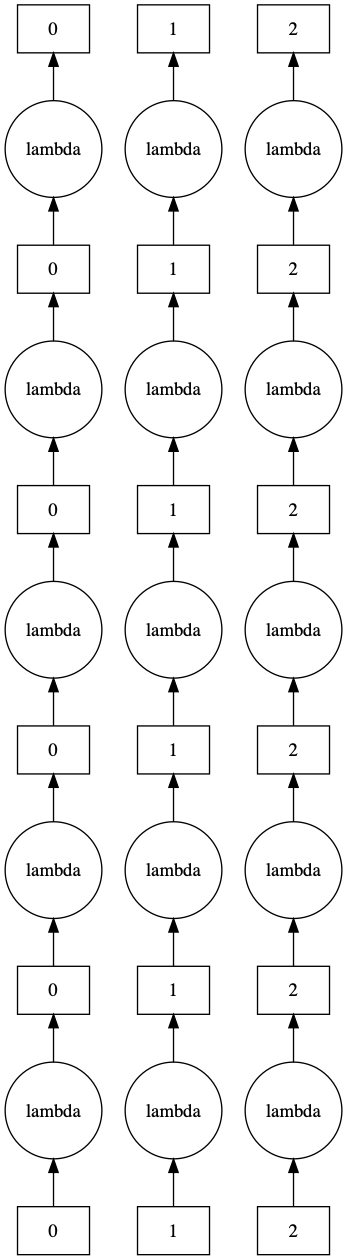
\includegraphics[height=\columnwidth,
    angle=-90]{images/incrementation-task-graph.png}
    \caption{Task graph for Incrementation with 5 iterations and 3 BigBrain blocks.
    Circles represent the incrementation and sleep function while rectangles
    represent data elements.}\label{fig:tg-inc}
\end{figure}

\subsubsection{Histogram}

 Our second application calculates the histogram of the BigBrain image (see
 Algorithm~\ref{alg:histogram}). It reads the image blocks from the shared
 file system, calculates intensity frequencies, aggregates the frequencies
 across the blocks, and finally writes the resulting histogram to the
 shared file system as a single \SI{766}{\kilo\byte} file. It follows the
 map-reduce paradigm, in which the final result is obtained from all the
 input blocks (see Fig.~\ref{fig:tg-histo}). This application requires data
 shuffling, incurring additional performance costs compared to
 Algorithm~\ref{alg:incrementation}. The total amount of shuffled data is,
 however, limited to \SI{2.62}{\mega\byte} per blocks as it only consists
 of image histograms. Two implementation are studied: a pure Python one,
 where frequencies are computed through Python dictionary manipulations, and one based
 on the \href{https://github.com/numpy}{NumPy} library, that implements array computations in C.

\begin{algorithm}[!t]
    \caption{Histogram}\label{alg:histogram}
    \begin{algorithmic}
    \Require{\(files\), files containing BigBrain blocks}
    \Require{\(fs\), NFS mount to save image to}
    \ForEach{\(file \in files\)}
        \State{Read \(block\) from \(file\)}
        \State{{Calculate \(frequencies\) in \(block\)}}
    \EndFor
    
    \State{\(histogram\gets\)Aggregate \(frequencies\) of each \(file\)}

    \State{Write \(histogram\) to \(fs\)}
    \end{algorithmic}
\end{algorithm}

\begin{figure}[!t]
    \centering
    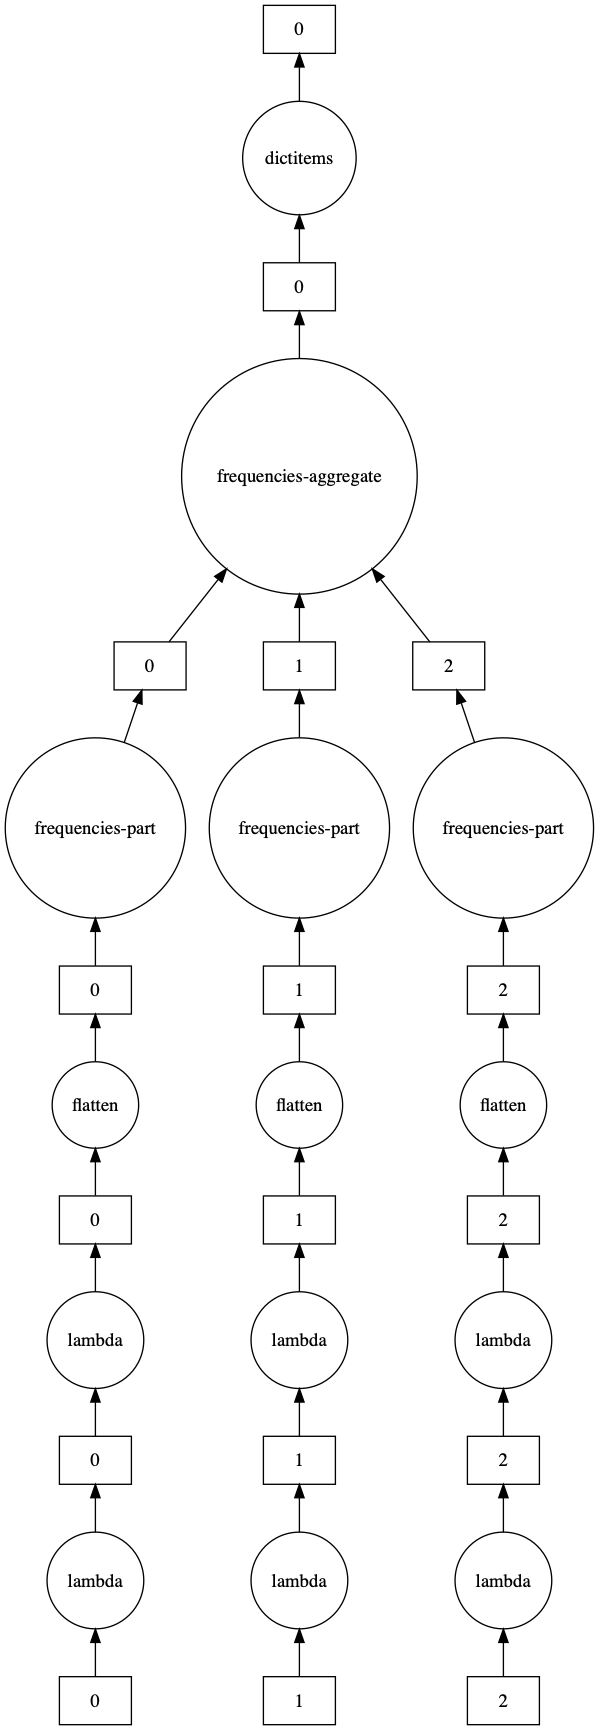
\includegraphics[height=\columnwidth,
    angle=-90]{images/histogram-task-graph.png}
    \caption{Task graph for Histogram with 3 BigBrain blocks. Circles represent the
    functions while rectangles represent data elements.
    }\label{fig:tg-histo}
\end{figure}

\subsubsection{BIDS app example}

We used the
\href{https://github.com/BIDS-Apps/example}{BIDS app example} map-reduce style 
application. The map phase, also called participant analysis, extracts the brain
tissues of a subject's 3D MRI from the CoRR dataset using the FMRIB Software Library
(\href{https://fsl.fmrib.ox.ac.uk/fsl/fslwiki}{FSL}), and writes the resulting
image (\SI{2.47}{\mega\byte} on average) to the NFS. The reduce phase, or group
analysis, computes the volume of each brain and returns the average
volume, shuffling a total of \SI{8.6}{\giga\byte} image data.

While Incrementation and Histogram were implemented directly in Python, the 
BIDS App example requires an external set of command-line tools distributed as a Docker container image
(bids/base\_fsl on DockerHub). We converted the Docker image to a Singularity image for use in 
an HPC environment, using
\href{https://hub.docker.com/r/singularityware/docker2singularity/tags/}{docker2singularity}.
The image was preloaded on the NFS and Singularity version 3.2.1\-1.el7 was installed
on all instances.

\subsection{Experiments}

Four parameters were varied in our experiments, as shown in
Table~\ref{tab:param}. We varied (1) the number of workers, to assess the
scalability of the engines, (2) the number of BigBrain blocks in
Incrementation and Histogram, to measure the effect of different I/O patterns
and parallelization degrees, and (3) the number of iterations and sleep
delay in Incrementation, to evaluate the effect of job length and number of
tasks.
It should be noted that increasing the number of blocks or iterations also
increases the total compute time of the application for a given sleep
delay. To avoid any potential external bias such as background load on the
network, we ran the experiments in a randomized order and cleared the page
cache of each worker before each execution.

For each run, we measured the application makespan as well as the cumulative 
data read, compute, data write, and engine overhead times across all application
tasks. 
The overhead calculation for each CPU is the end time of its last processed task
minus the start time of the application. The summation of those results is the
total overhead. \TG{This last sentence looks wrong to me.}

% The baseline for our experiments is: 8 workers, 125 blocks, 10 iterations and 4
% seconds sleep delay.

\begin{table}[!t]
    \renewcommand{\arraystretch}{1.3}
    \caption{Parameters for the experiments}\label{tab:param}
    \centering
    \begin{tabular*}{\columnwidth}{llll}
    \hline
                        & Incrementation & Histogram             & BIDS Example          \\ \hline
    \# of worker        & 1, 2, 4, 8     & 1, 2, 4, 8            & 1, 2, 4, 8            \\
    \# of blocks        & 30, 125, 750   & 30, 125, 750          & \multicolumn{1}{c}{-} \\
    \# of iterations    & 1, 10, 100     & \multicolumn{1}{c}{-} & \multicolumn{1}{c}{-} \\
    Sleep delay {[}\SI{}{\second}{]} & 1, 4, 16, 64   & \multicolumn{1}{c}{-} & \multicolumn{1}{c}{-} \\ \hline
    \end{tabular*}
    \end{table}






%%%%% RESULTS %%%%%
\section{Results}

%%% INCREMENTATION %%%
%% worker
\subsection{Incrementation: Number of workers}
Figure~\ref{fig:inc_ms_worker} shows the makespan of the Incrementation application
for different numbers of workers and engines. The bars show the average
makespan over 3 repetitions while the error bars are the standard deviations. Overall,
there is no substantial makespan difference between the engines. Dask seems to have a
slight advantage over Spark, \SI{83.61}{\second} on average,
with Delayed and Futures being slightly better than Bag.

For all engines, the makespan is far from decreasing linearly with the
number of workers. The makespan
even increases between 4 and 8 workers. This is due to the high impact of
data transfers and engine overhead on the application. 

Figure~\ref{fig:inc_tt_worker} shows the total execution time of the
Incrementation application, broken down into data transfer (read and
write), compute (sleep), and overhead time. As expected, the computing time
stays similar when the number of workers increases. However, the data
transfer time and overhead increase substantially with the number of
workers.

% \hspace{1cm}\(\hat{y}=2336.9499\cdot{x} + 325.00574\) (Spark)

% \hspace{1cm}\(\hat{y}=2650.13505\cdot{x} + 1585.37218\) (Bag)

% \hspace{1cm}\(\hat{y}=3250.53406\cdot{x} + 1769.50351\) (Delayed)

% \hspace{1cm}\(\hat{y}=3570.39758\cdot{x} + 1062.23031\) (Futures)

On Figure~\ref{fig:inc_tt_worker}, we also note that Spark's overhead is
slightly lower than Dask's, particularly when the number of workers
increase. Moreover, Delayed and Futures have a higher overhead than Bag.
However, overhead differences are compensated by an increase in data
transfer time, as a reduced overhead increases the concurrency between data
transfers and the application saturates the 10Gbits/s network bandwidth. 

\begin{figure}[!b]
    \centering
    \begin{subfigure}[b]{\columnwidth}
        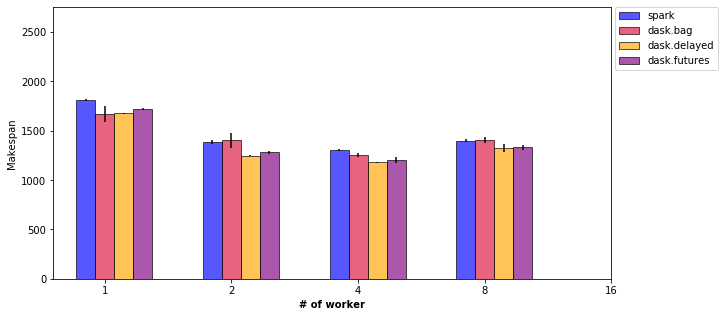
\includegraphics[clip,width=\columnwidth]{images/inc_worker.png}%
        \caption{Incrementation makespan}\label{fig:inc_ms_worker}
    \end{subfigure}
    \\
    \begin{subfigure}[b]{\columnwidth}
        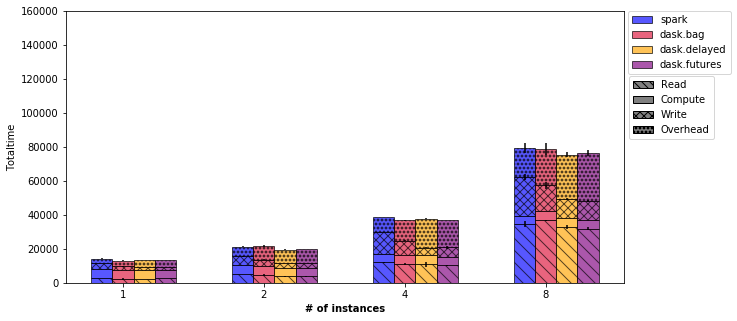
\includegraphics[clip,width=\columnwidth]{images/inc_idle_worker.png}%
        \caption{Incrementation total time}\label{fig:inc_tt_worker}
    \end{subfigure}
    \caption{125 blocks, 10 iterations, \SI{4}{\second} delay, 8
    CPUs/worker}\label{fig:inc_worker}
\end{figure}

% blocks
\subsection{Incrementation: Number of blocks}

Figure~\ref{fig:inc_ms_block} shows the Incrementation makespan when varying the
number of image blocks for constant BigBrain image size. We were not able to run
Spark for 30 blocks due to its \SI{2}{\giga\byte} limitation in the task size.
 Once again, we do not observe any substantial difference among the engines.
For all engines, makespan variability increases with the number of blocks, however,
engines scale very well in general.


In Figure~\ref{fig:inc_tt_block}, the total execution time of each function is shown.
For 30 blocks, the increased overhead of Delayed and Futures is a calculation artifact 
coming from the fact that only 30 of the 64 available threads can be used concurrently. Once again, the data transfer time reduces with more blocks but 
the overhead time increases by a similar amount. This is not observed for 30 blocks
as the workers are not used at full capacity, i.e., some threads are idle. Finally,
the variability of the overhead increases with the number of blocks, which explains
the makespan variability mentioned previously.

\begin{figure}[!t]
    \centering
    \begin{subfigure}[b]{\columnwidth}
        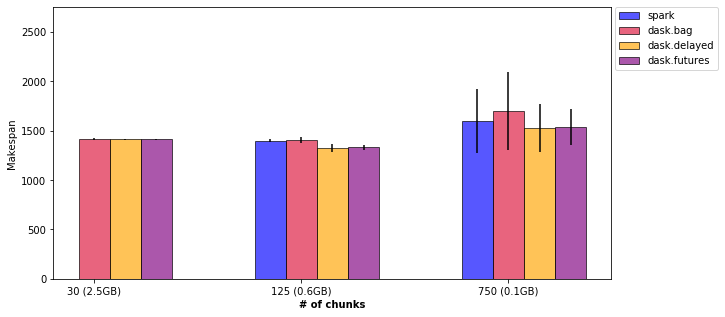
\includegraphics[clip,width=\columnwidth]{images/inc_block.png}%
        \caption{Incrementation makespan}\label{fig:inc_ms_block}
    \end{subfigure}
    \\
    \begin{subfigure}[b]{\columnwidth}
        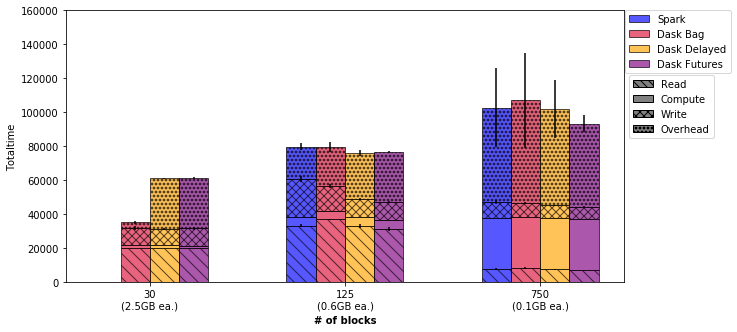
\includegraphics[clip,width=\columnwidth]{images/inc_idle_block.png}%
        \caption{Incrementation total time}\label{fig:inc_tt_block}
    \end{subfigure}
    \caption{10 iterations, \SI{4}{\second} delay, 8 workers, 8
    CPUs/worker}\label{fig:inc_block}
\end{figure}

%% Iterations
\subsection{Incrementation: Number of iterations}
Figure~\ref{fig:inc_ms_itr} shows the makespan of the application while
varying the number of iterations. Overall, Spark and Dask APIs are once
again equivalent, although Delayed and Futures are slightly faster
than Bag and Spark for 1 and 10 iterations, and Futures are faster than
Delayed, Bag and Spark for 100 iterations. Differences remain minor
though.

In Figure~\ref{fig:inc_tt_itr}, the total execution time breakdown is
shown. We observe the good scalability of all the engines with the number of
iterations.


\begin{figure}[!t]
    \centering
    \begin{subfigure}[b]{\columnwidth}
        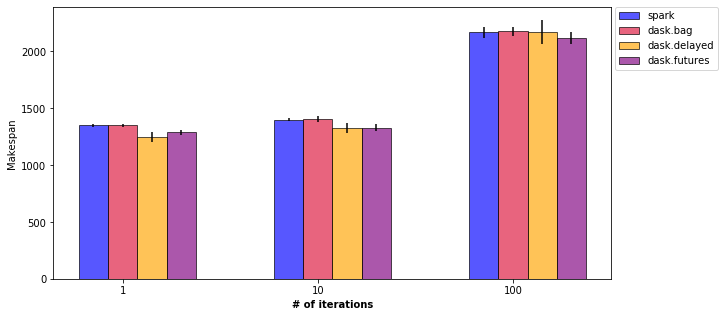
\includegraphics[clip,width=\columnwidth]{images/inc_itr.png}%
        \caption{Incrementation makespan}\label{fig:inc_ms_itr}
    \end{subfigure}
    \\
    \begin{subfigure}[b]{\columnwidth}
        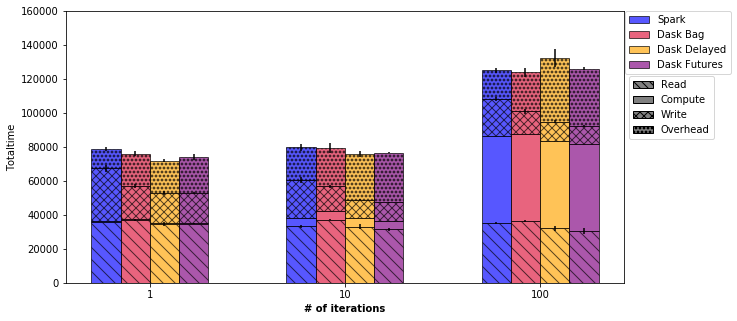
\includegraphics[clip,width=\columnwidth]{images/inc_idle_itr.png}%
        \caption{Incrementation total time}\label{fig:inc_tt_itr}
    \end{subfigure}
    \caption{125 blocks, \SI{4}{\second} delay, 8 workers, 8 CPUs/worker}
\end{figure}

%% Sleep time
\subsection{Incrementation: Sleep delay}
Figure~\ref{fig:inc_ms_sleep} shows the makespan of the Incrementation application
for different sleep delays. Overall, all engines again perform the same and scale
well with task duration. Spark is initially slower than the Dask APIs, however, it is
faster with an increased sleep delay. Also, within the Dask APIs, Dask Bag is
slower than the other two, but it is not considerable.

Figure~\ref{fig:inc_tt_sleep} shows the total execution time breakdown. Spark has the
smallest overhead. As previously observed, variations in overhead time are almost
exactly compensated by variations in data transfer time.

\begin{figure}[!b]
    \centering
    \begin{subfigure}[b]{\columnwidth}
        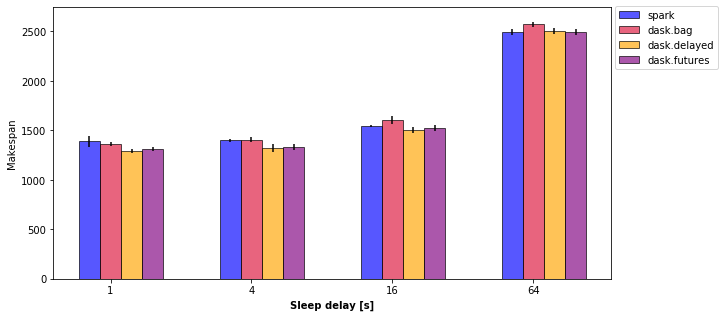
\includegraphics[clip,width=\columnwidth]{images/inc_sleep.png}%
        \caption{Incrementation makespan}\label{fig:inc_ms_sleep}
    \end{subfigure}
    \\
    \begin{subfigure}[b]{\columnwidth}
        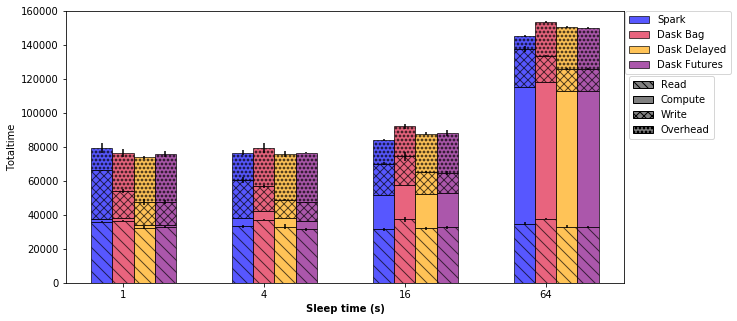
\includegraphics[clip,width=\columnwidth]{images/inc_idle_sleep.png}%
        \caption{Incrementation total time}\label{fig:inc_tt_sleep}
    \end{subfigure}
    \caption{125 blocks, 10 iterations, 8 workers, 8 CPUs/worker}
\end{figure}

%% Baseline gantt chart
\subsection{Incrementation: Gantt chart}

Figure~\ref{fig:inc_gantt} shows the Gantt chart obtained for each engine. Gantt
charts are structured in batches of up to 64 read-compute-write concurrent sequences.
File reads in the first batch are much longer than the ones in the following batches:
this is due to the high synchronization of data transfers that leads to a high
saturation of the shared file system. We also note that overhead, represented in
white, is concentrated around the data transfer tasks and the
computing tasks that run concurrently with data transfers. 

\begin{figure}[!b]
    \centering
    \begin{subfigure}[b]{\columnwidth}
        \href{https://zenodo.org/record/3354434/files/spark-inc-baseline.html?download=1}{
            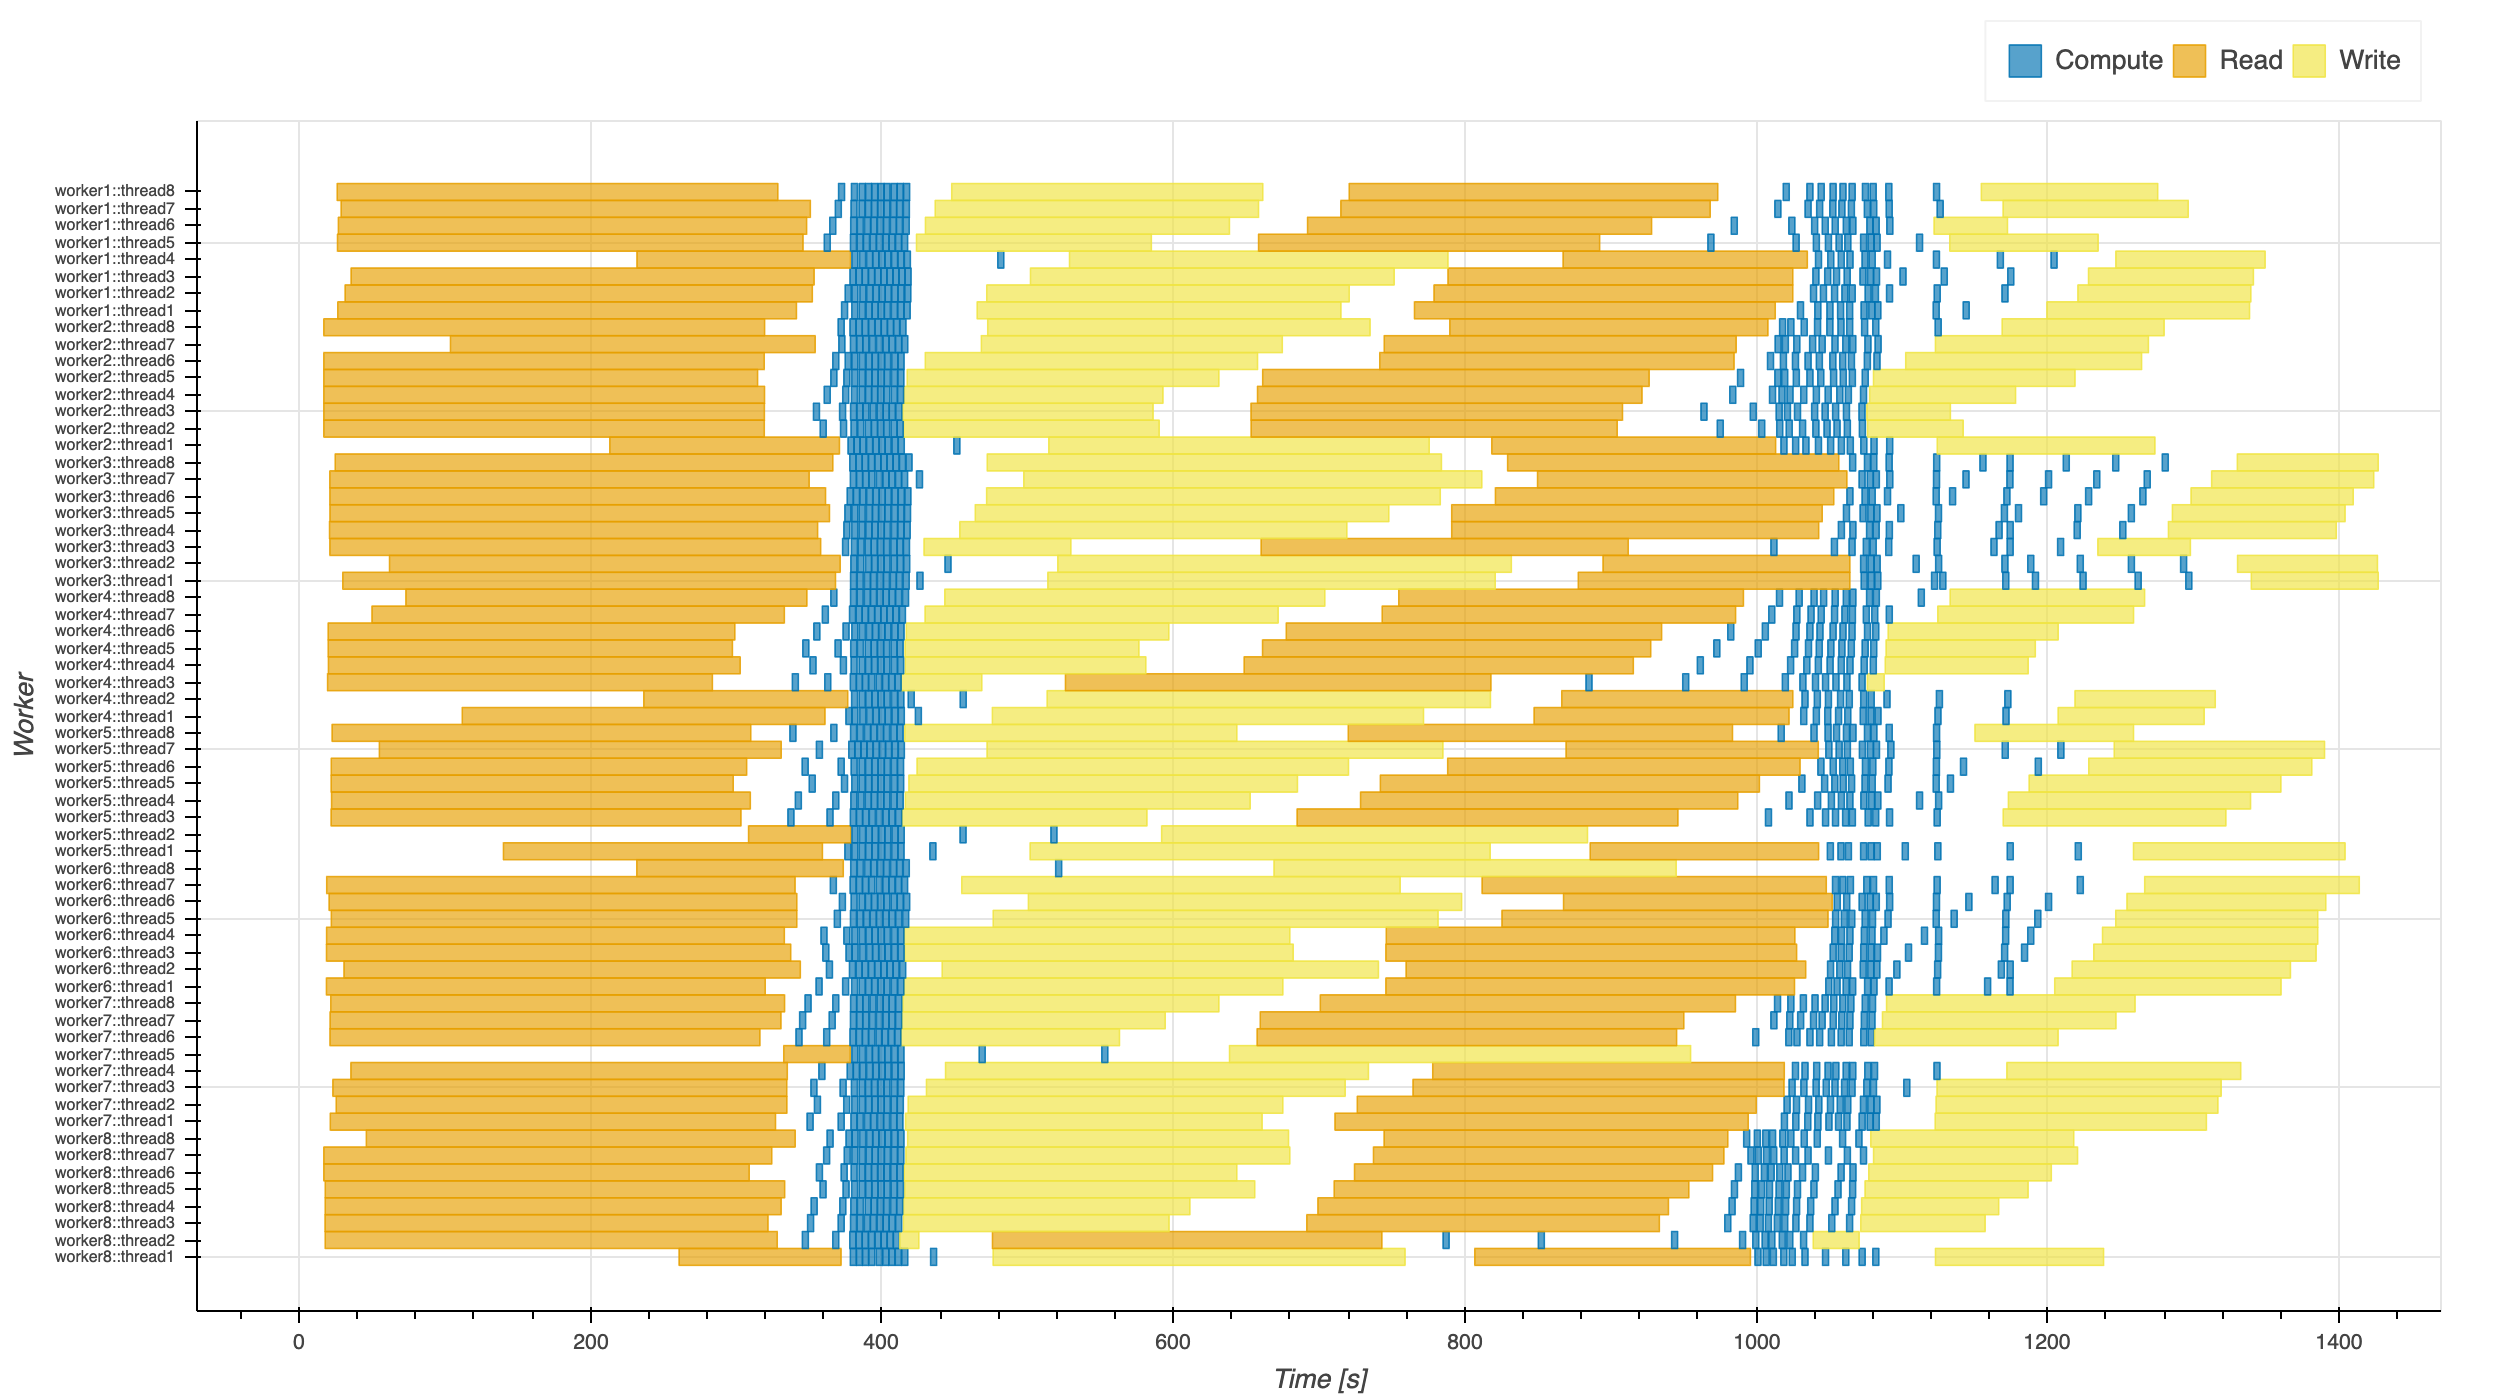
\includegraphics[clip,width=\columnwidth,
            height=0.15\textheight]{images/spark_inc_gantt.png}}
        \caption{Spark}\label{fig:inc_spark_gantt}
    \end{subfigure}
    \\
    \begin{subfigure}[b]{\columnwidth}
        \href{https://zenodo.org/record/3354434/files/dask-bag-inc-baseline.html?download=1}{
        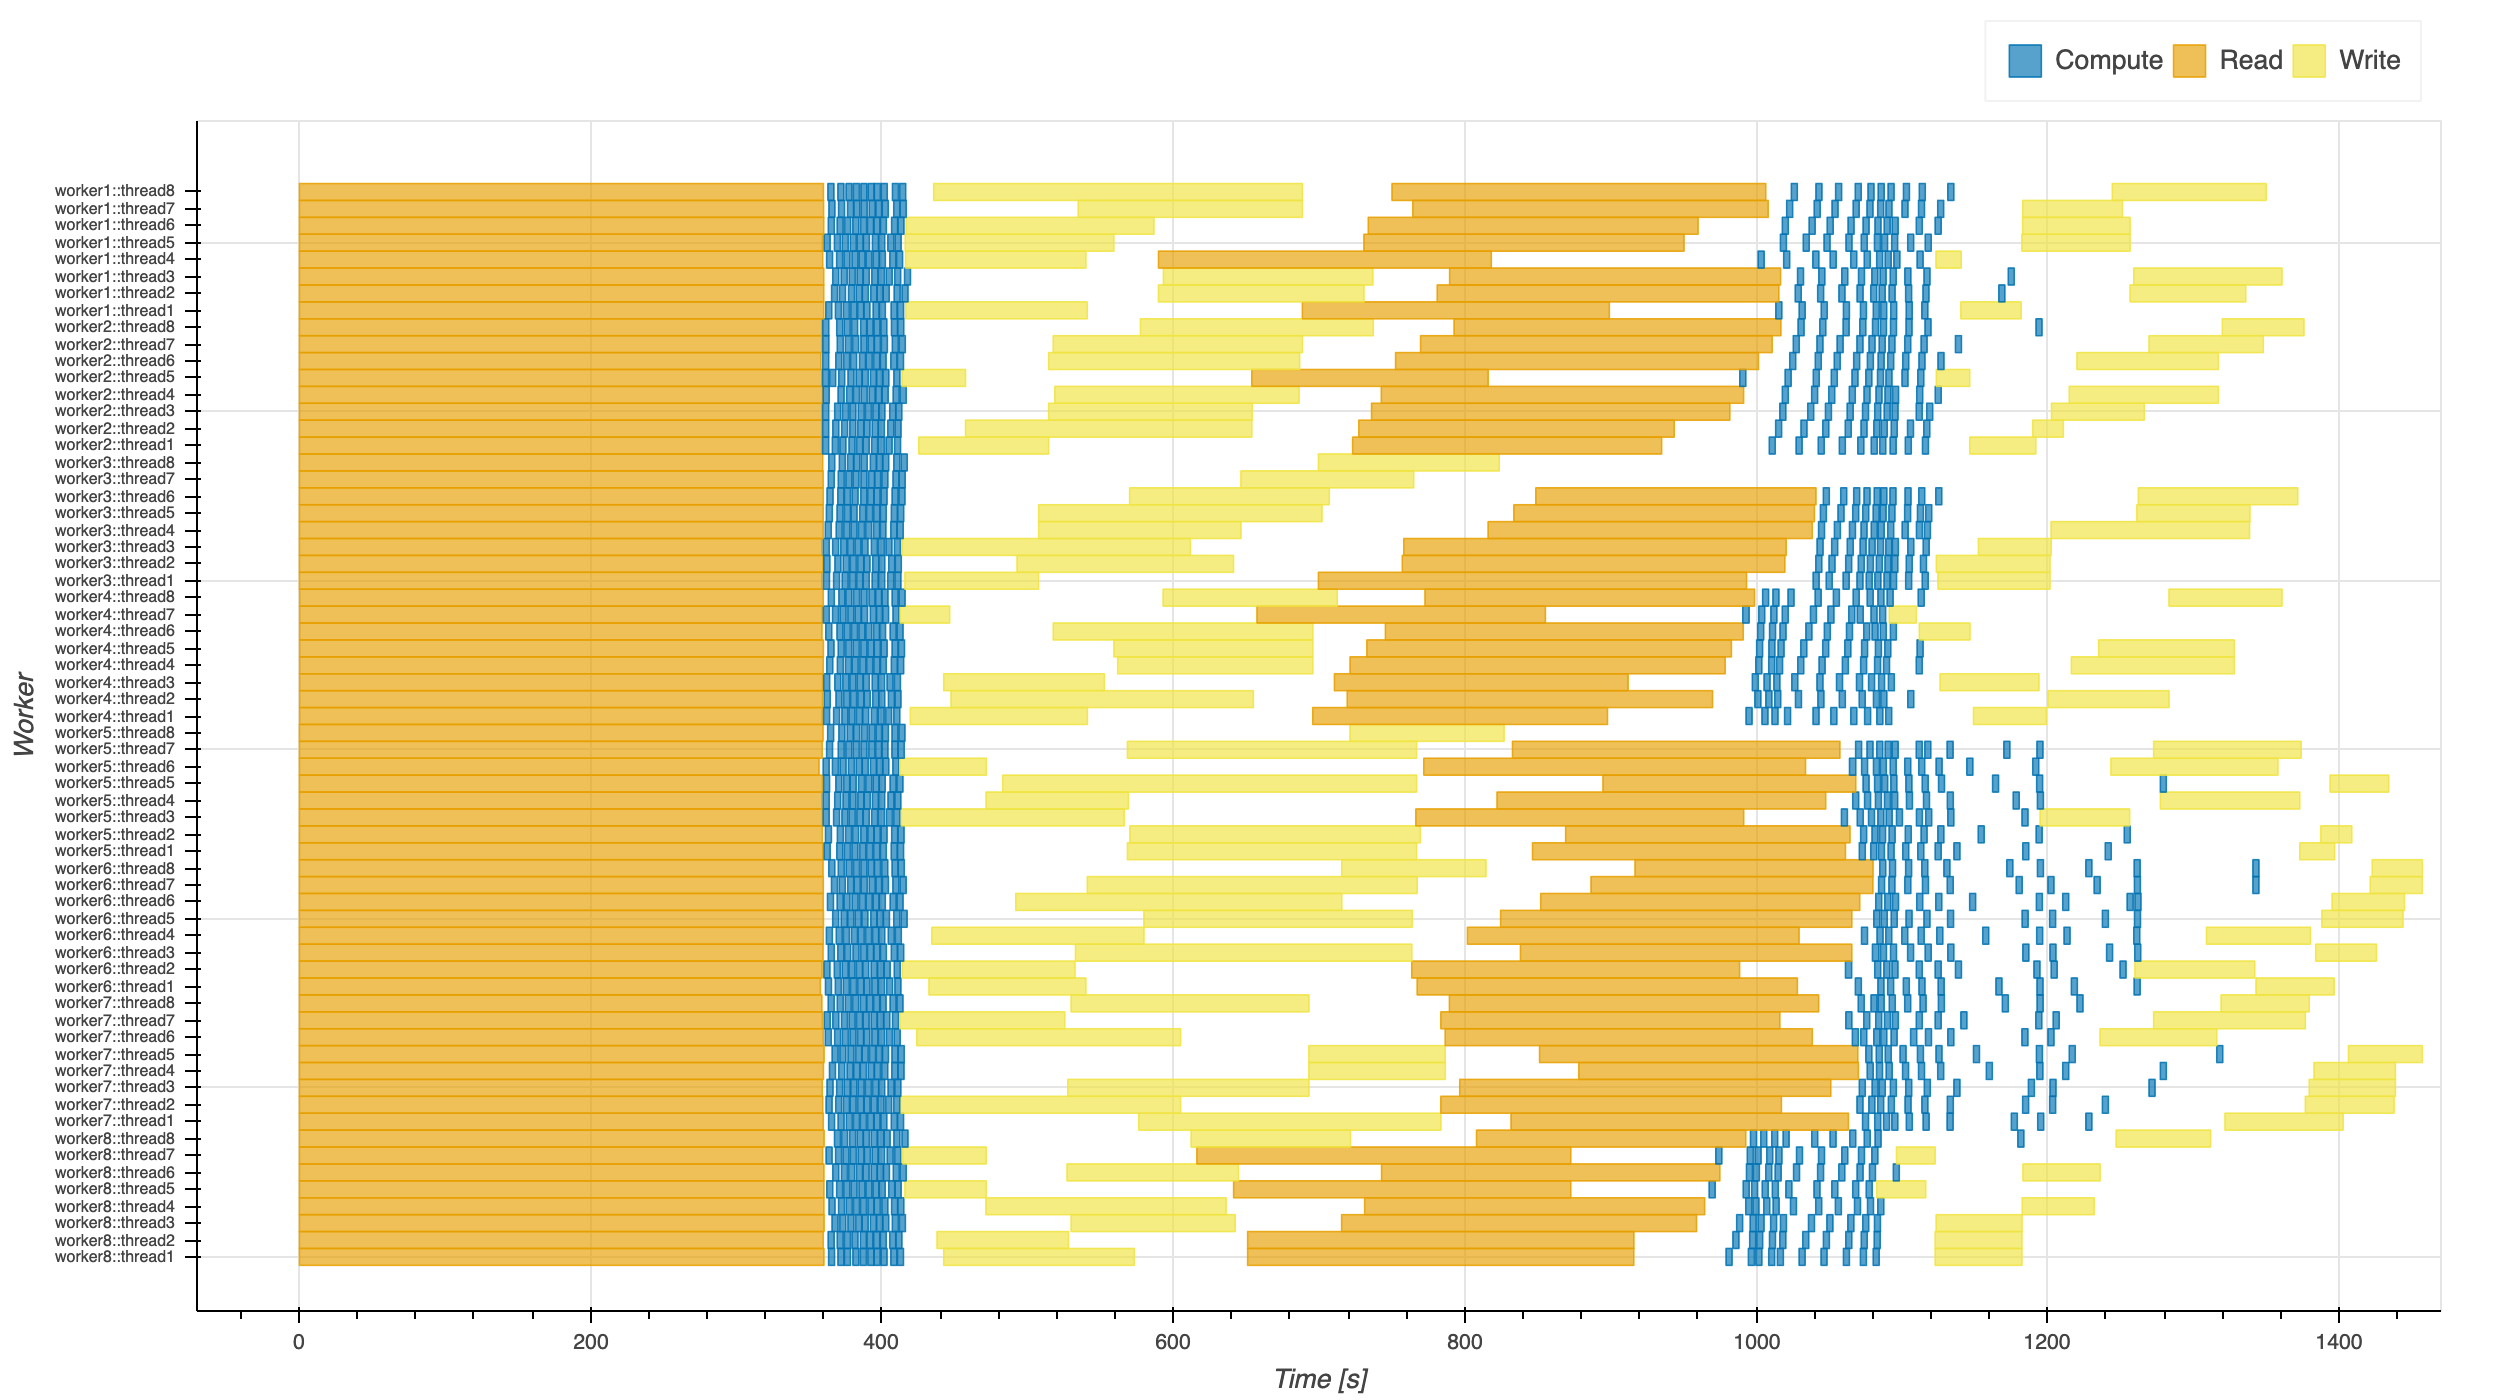
\includegraphics[clip,width=\columnwidth,
        height=0.15\textheight]{images/bag_inc_gantt.png}}
        \caption{Dask Bag}\label{fig:inc_dask_bag_gantt}
    \end{subfigure}
    \\
    \begin{subfigure}[b]{\columnwidth}
        \href{https://zenodo.org/record/3354434/files/dask-delayed-inc-baseline.html?download=1}{
        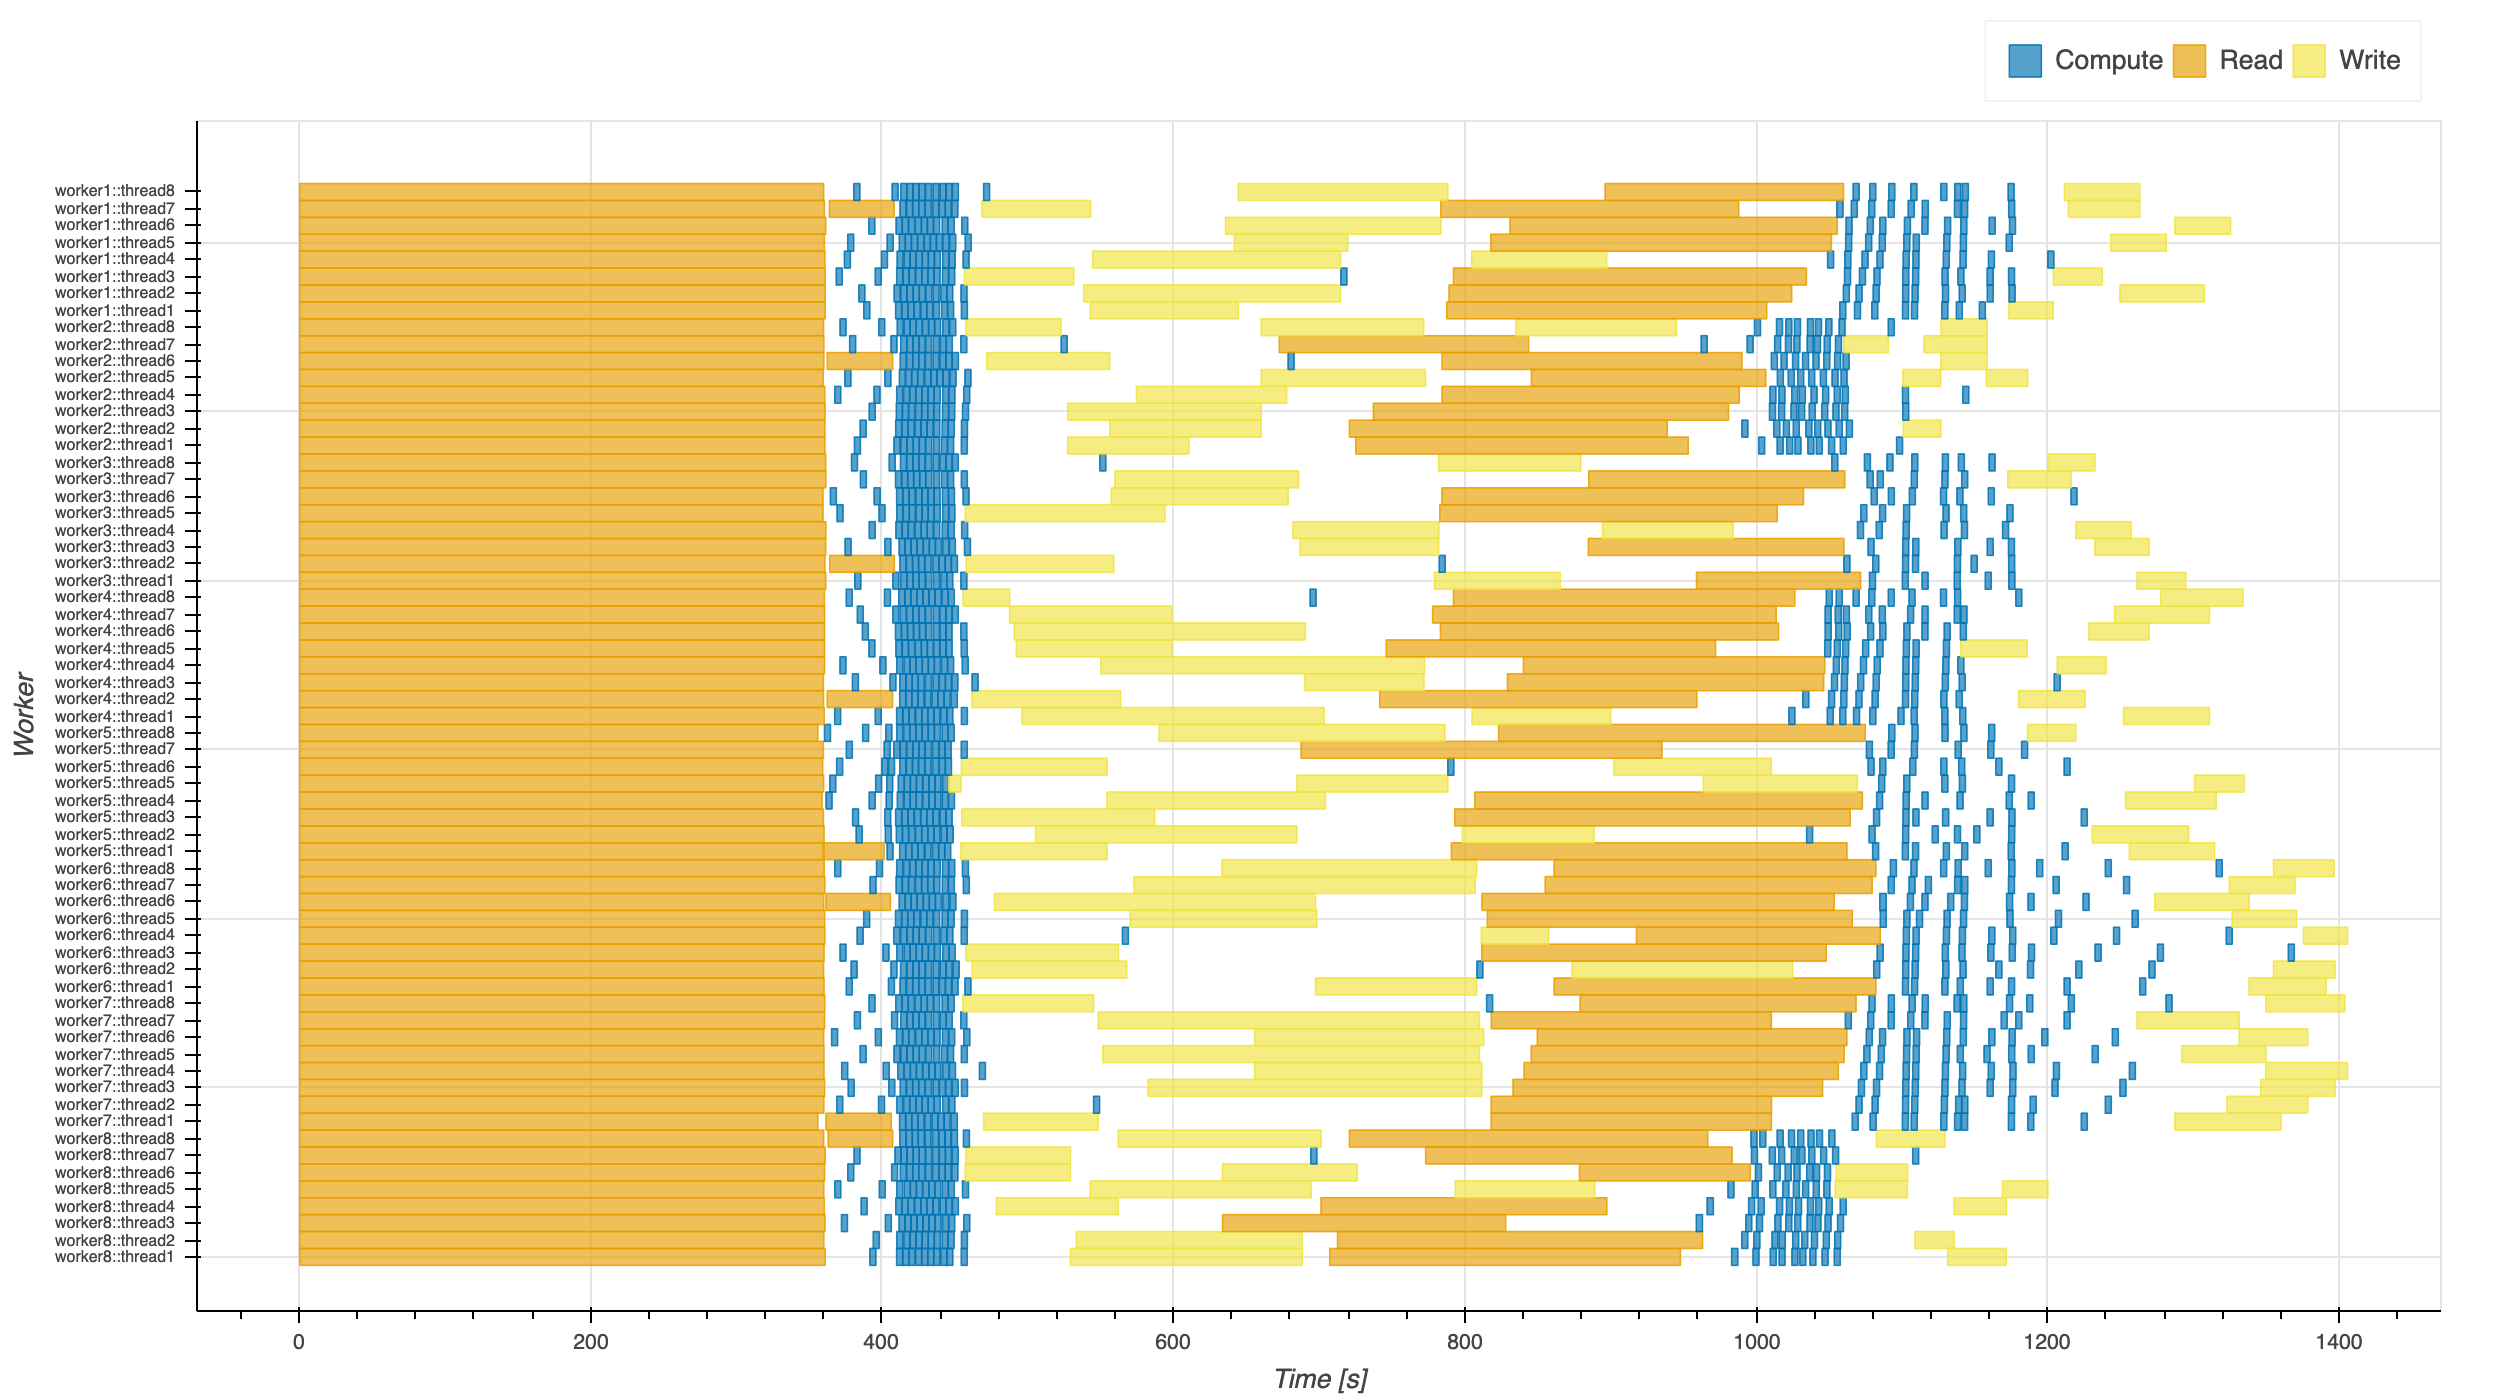
\includegraphics[clip,width=\columnwidth,
        height=0.15\textheight]{images/delayed_inc_gantt.png}}
        \caption{Dask Delayed}\label{fig:inc_dask_delayed_gantt}
    \end{subfigure}
    \\
    \begin{subfigure}[b]{\columnwidth}
        \href{https://zenodo.org/record/3354434/files/dask-futures-inc-baseline.html?download=1}{
        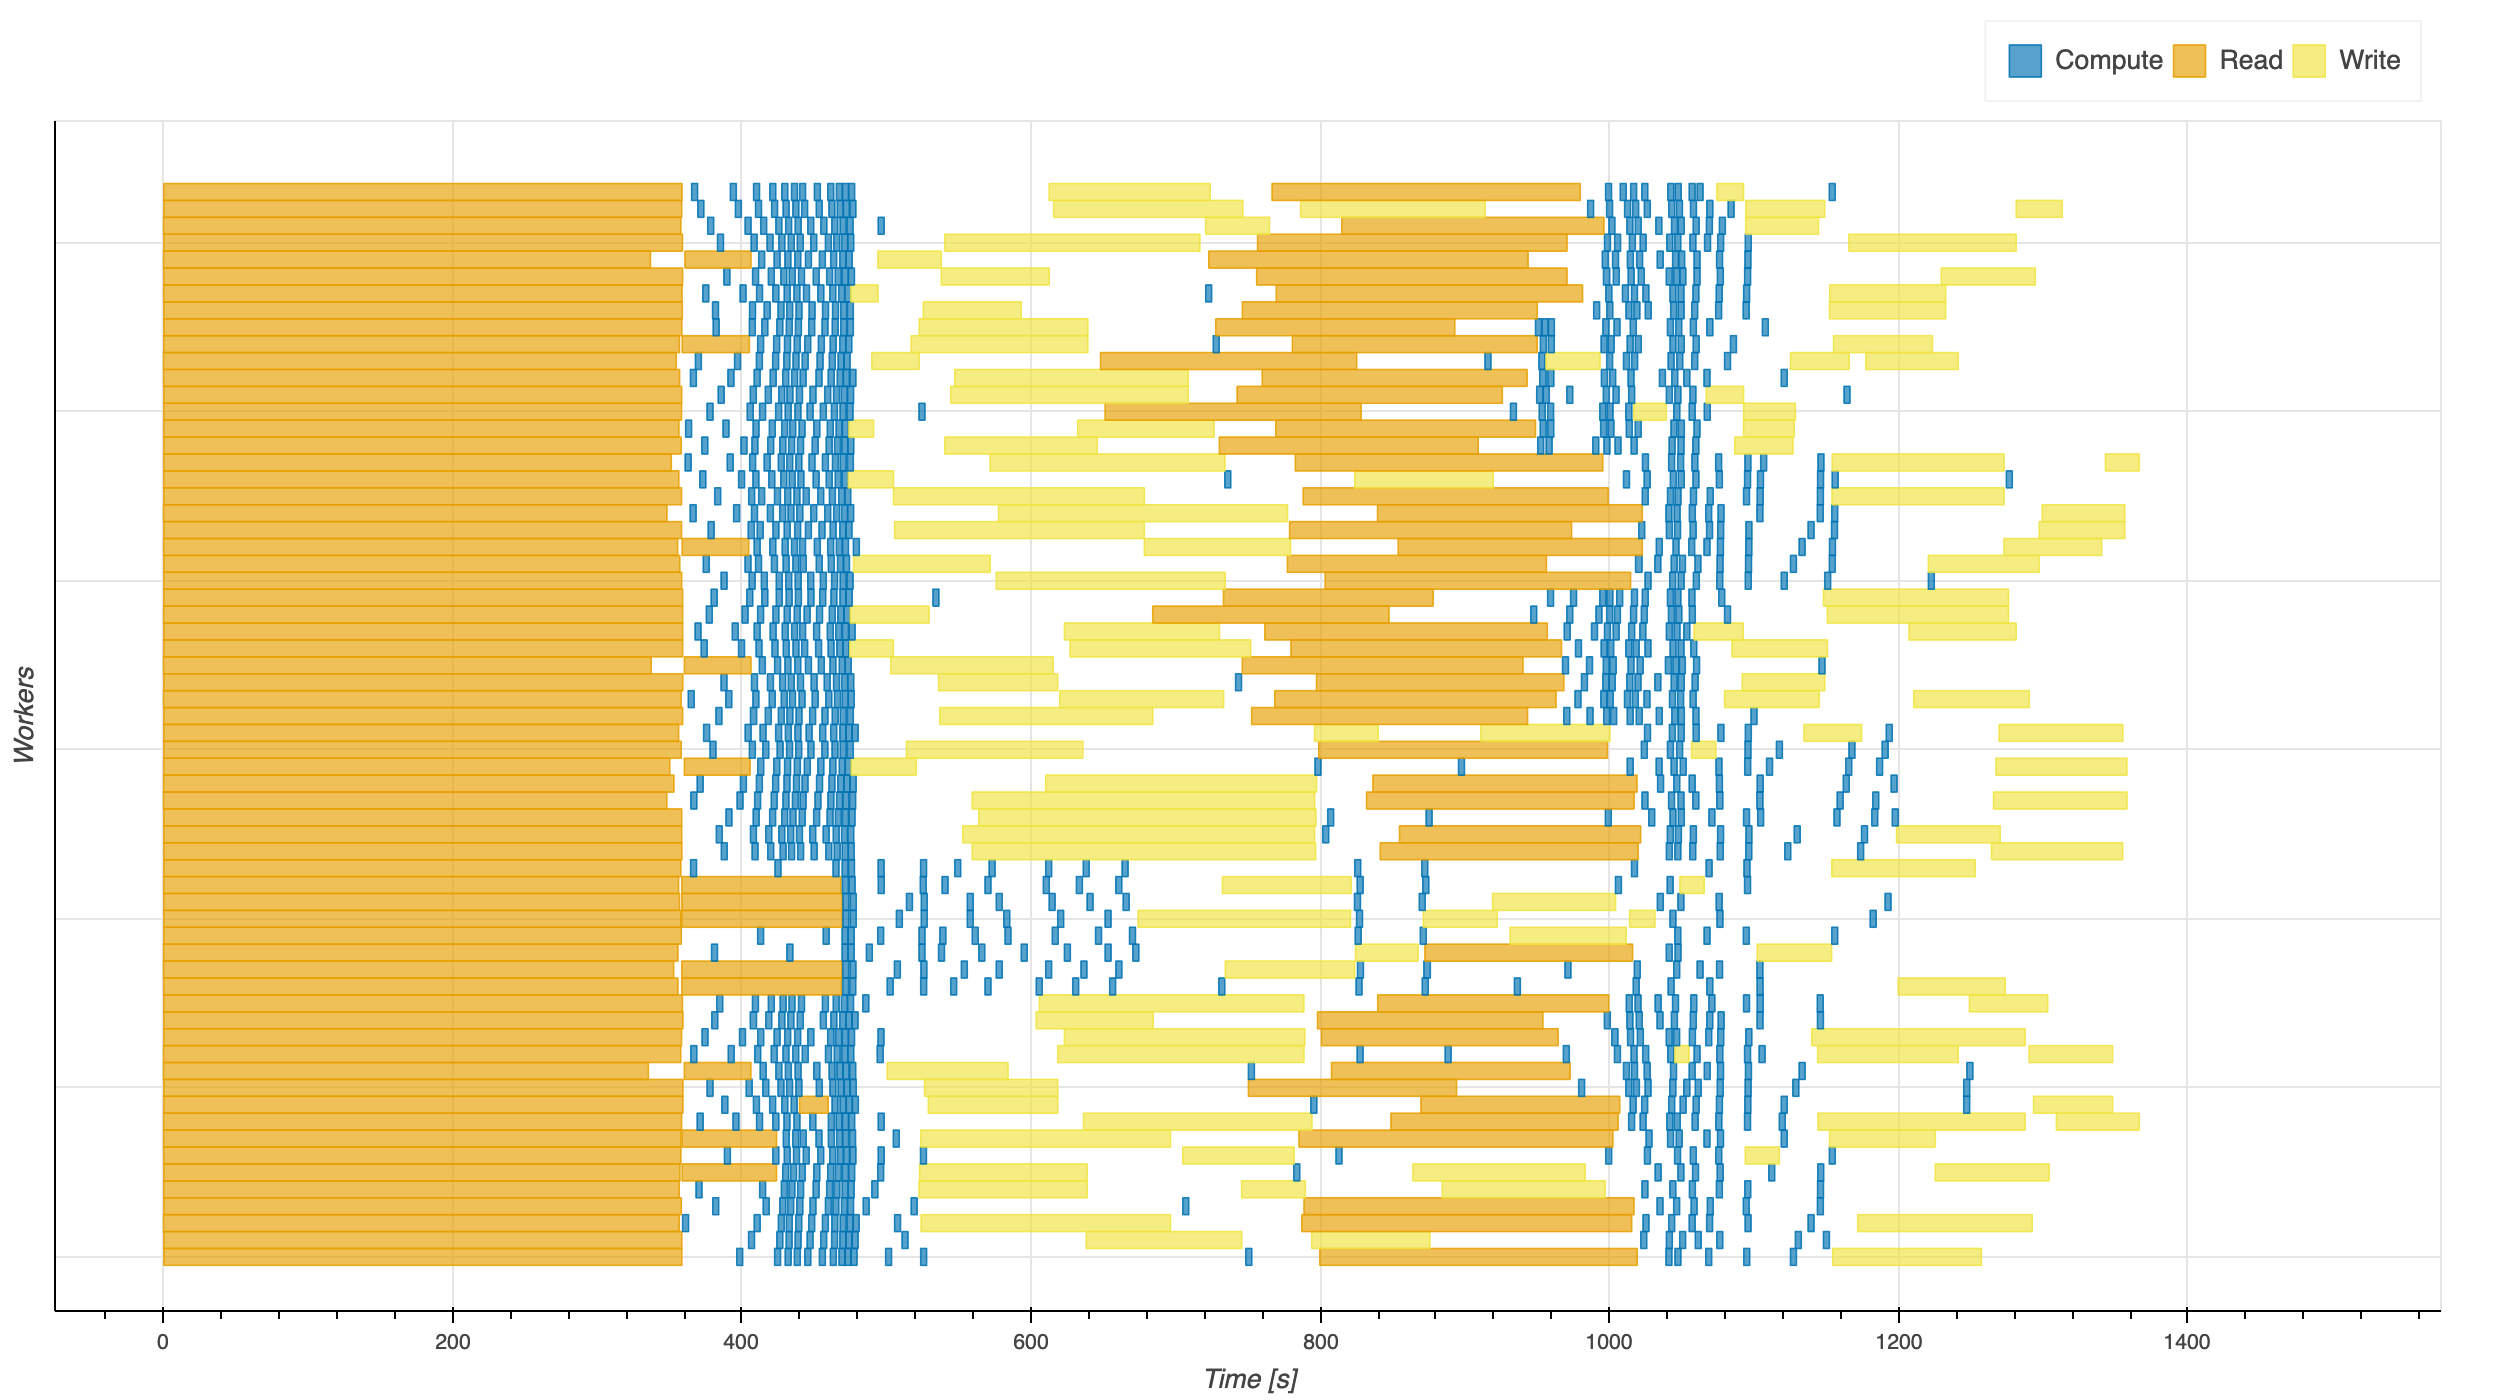
\includegraphics[clip,width=\columnwidth,
        height=0.15\textheight]{images/futures_inc_gantt.png}}
        \caption{Dask Futures}\label{fig:inc_dask_futures_gantt}
    \end{subfigure}
    \caption{Incrementation: 125 blocks, 10 iterations, \SI{4}{\second} delay, 8 workers,
8 CPUs/worker}\label{fig:inc_gantt}
\end{figure}

%%% HISTOGRAM %%%
\subsection{Histogram (Python): Number of workers}
Figure~\ref{fig:histo_ms_worker} shows the makespan of the Histogram application for various
amounts of workers. Spark is significantly faster than Dask APIs. The difference
narrows as the number of workers increases but it remains significant. Between Dask APIs
there is no substantial difference, however, Bag is slightly faster on average.

From Figure~\ref{fig:histo_tt_worker}, the total time spent in each function is
shown. The compute time is significantly larger for Dask than for Spark. This is
presumably due to Python's GIL preventing Dask to parallelize the computation
over
multiple threads. Overall, the I/O and overhead times are comparable for all engines.

Figure~\ref{fig:histo_tt_worker} shows that Dask engines have a similar
total execution time when their number of workers varies, except for 8
workers where it increases slightly due to increased read time.
On the other hand, Spark total execution time keeps increasing; especially at 8
workers. This is because Dask engines benefit more from additional workers, in
this GIL-bounded scenario.

\begin{figure}[!b]
    \centering
    \begin{subfigure}[b]{\columnwidth}
        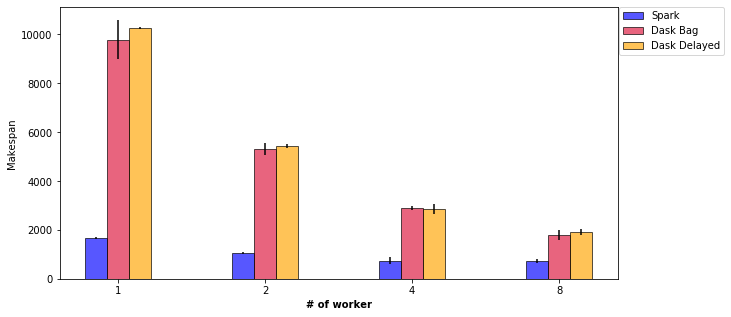
\includegraphics[clip,width=\columnwidth]{images/histo_worker.png}%
        \caption{Histogram (Python) makespan}\label{fig:histo_ms_worker}
    \end{subfigure}
    \\
    \begin{subfigure}[b]{\columnwidth}
        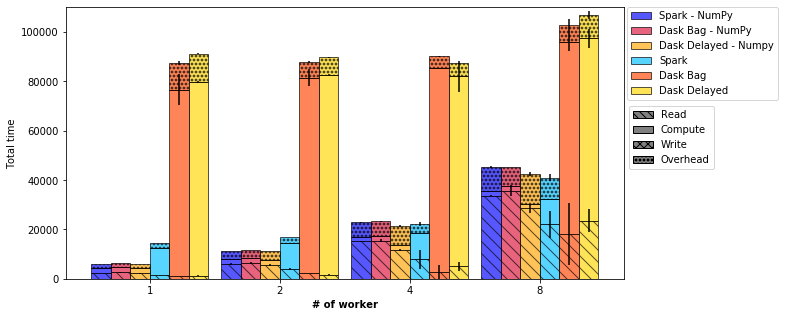
\includegraphics[clip,width=\columnwidth]{images/histo_idle_worker.png}%
        \caption{Histogram (Python) total time}\label{fig:histo_tt_worker}
    \end{subfigure}
    \caption{125 blocks, 8 CPUs/worker}
\end{figure}

\subsection{Histogram (Python): Number of blocks}
Figure~\ref{fig:histo_ms_block} shows the makespan for different block sizes. 
Once more, Spark is significantly faster than Dask engines and Bag is slightly
faster than Delayed. Overall, the engines do not react to changes in block size.

In Figure~\ref{fig:histo_tt_block} the total time for each function is shown.
Note that at 30 blocks the workers' resources are not fully used since the
workers can process up to 64 tasks in parallel. Moreover, the overhead for
30 blocks is erroneous due to a lower amount of block than available threads.
This leads to thread based engines to have higher overhead. Given that, 
Spark has a much lower compute time which makes it significantly faster
than Dask engines. Overall, for all engines, lower block size results in lower
IO time but increases the overhead time. Again, this is due to large overhead
desynchronizing task thus reducing the NFS bottleneck.


\begin{figure}[!t]
    \centering
    \begin{subfigure}[b]{\columnwidth}
        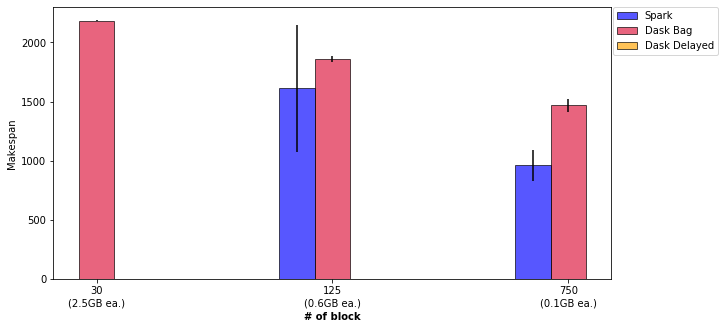
\includegraphics[clip,width=\columnwidth]{images/histo_block.png}%
        \caption{Histogram (Python) makespan}\label{fig:histo_ms_block}
    \end{subfigure}
    \\
    \begin{subfigure}[b]{\columnwidth}
        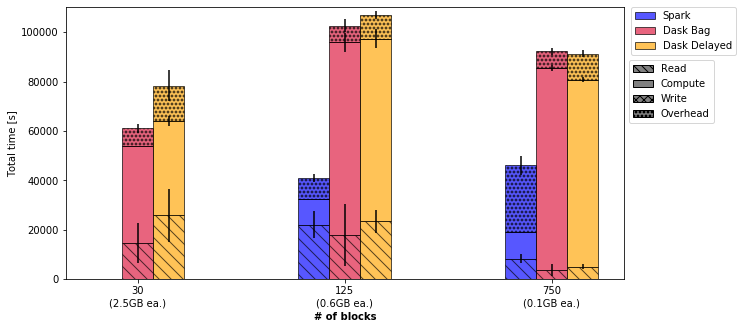
\includegraphics[clip,width=\columnwidth]{images/histo_idle_block.png}%
        \caption{Histogram (Python) total time}\label{fig:histo_tt_block}
    \end{subfigure}
    \caption{8 workers, 8 CPUs/worker}
\end{figure}
% \TG{We decided to omit Dask Futures as it does not have any value over Dask
% Delayed in this application.}

\subsection{Histogram (Python): Gantt chart}
Figure~\ref{fig:histo_gantt} shows the Gantt chart of the baseline
Histogram experiment implemented in Python. Spark overhead is distributed
through all the execution while Bag overhead happens mostly when a thread
reads subsequent blocks and Delayed overhead is concentrated after reading
all the blocks.

% % remove? - vhs
% The reduce is done differently for the engines. Spark and Delayed compute
% all the reduce tasks on one process (thread), however, Spark only computes it
% on the driver process. On the other hand, Bag computes the reduce tasks on 
% different workers and sends the information to the driver process afterward.

\begin{figure}[!t]
    \centering
    \begin{subfigure}[b]{\columnwidth}
        \href{https://zenodo.org/record/3354434/files/spark-histo-baseline.html?download=1}{
        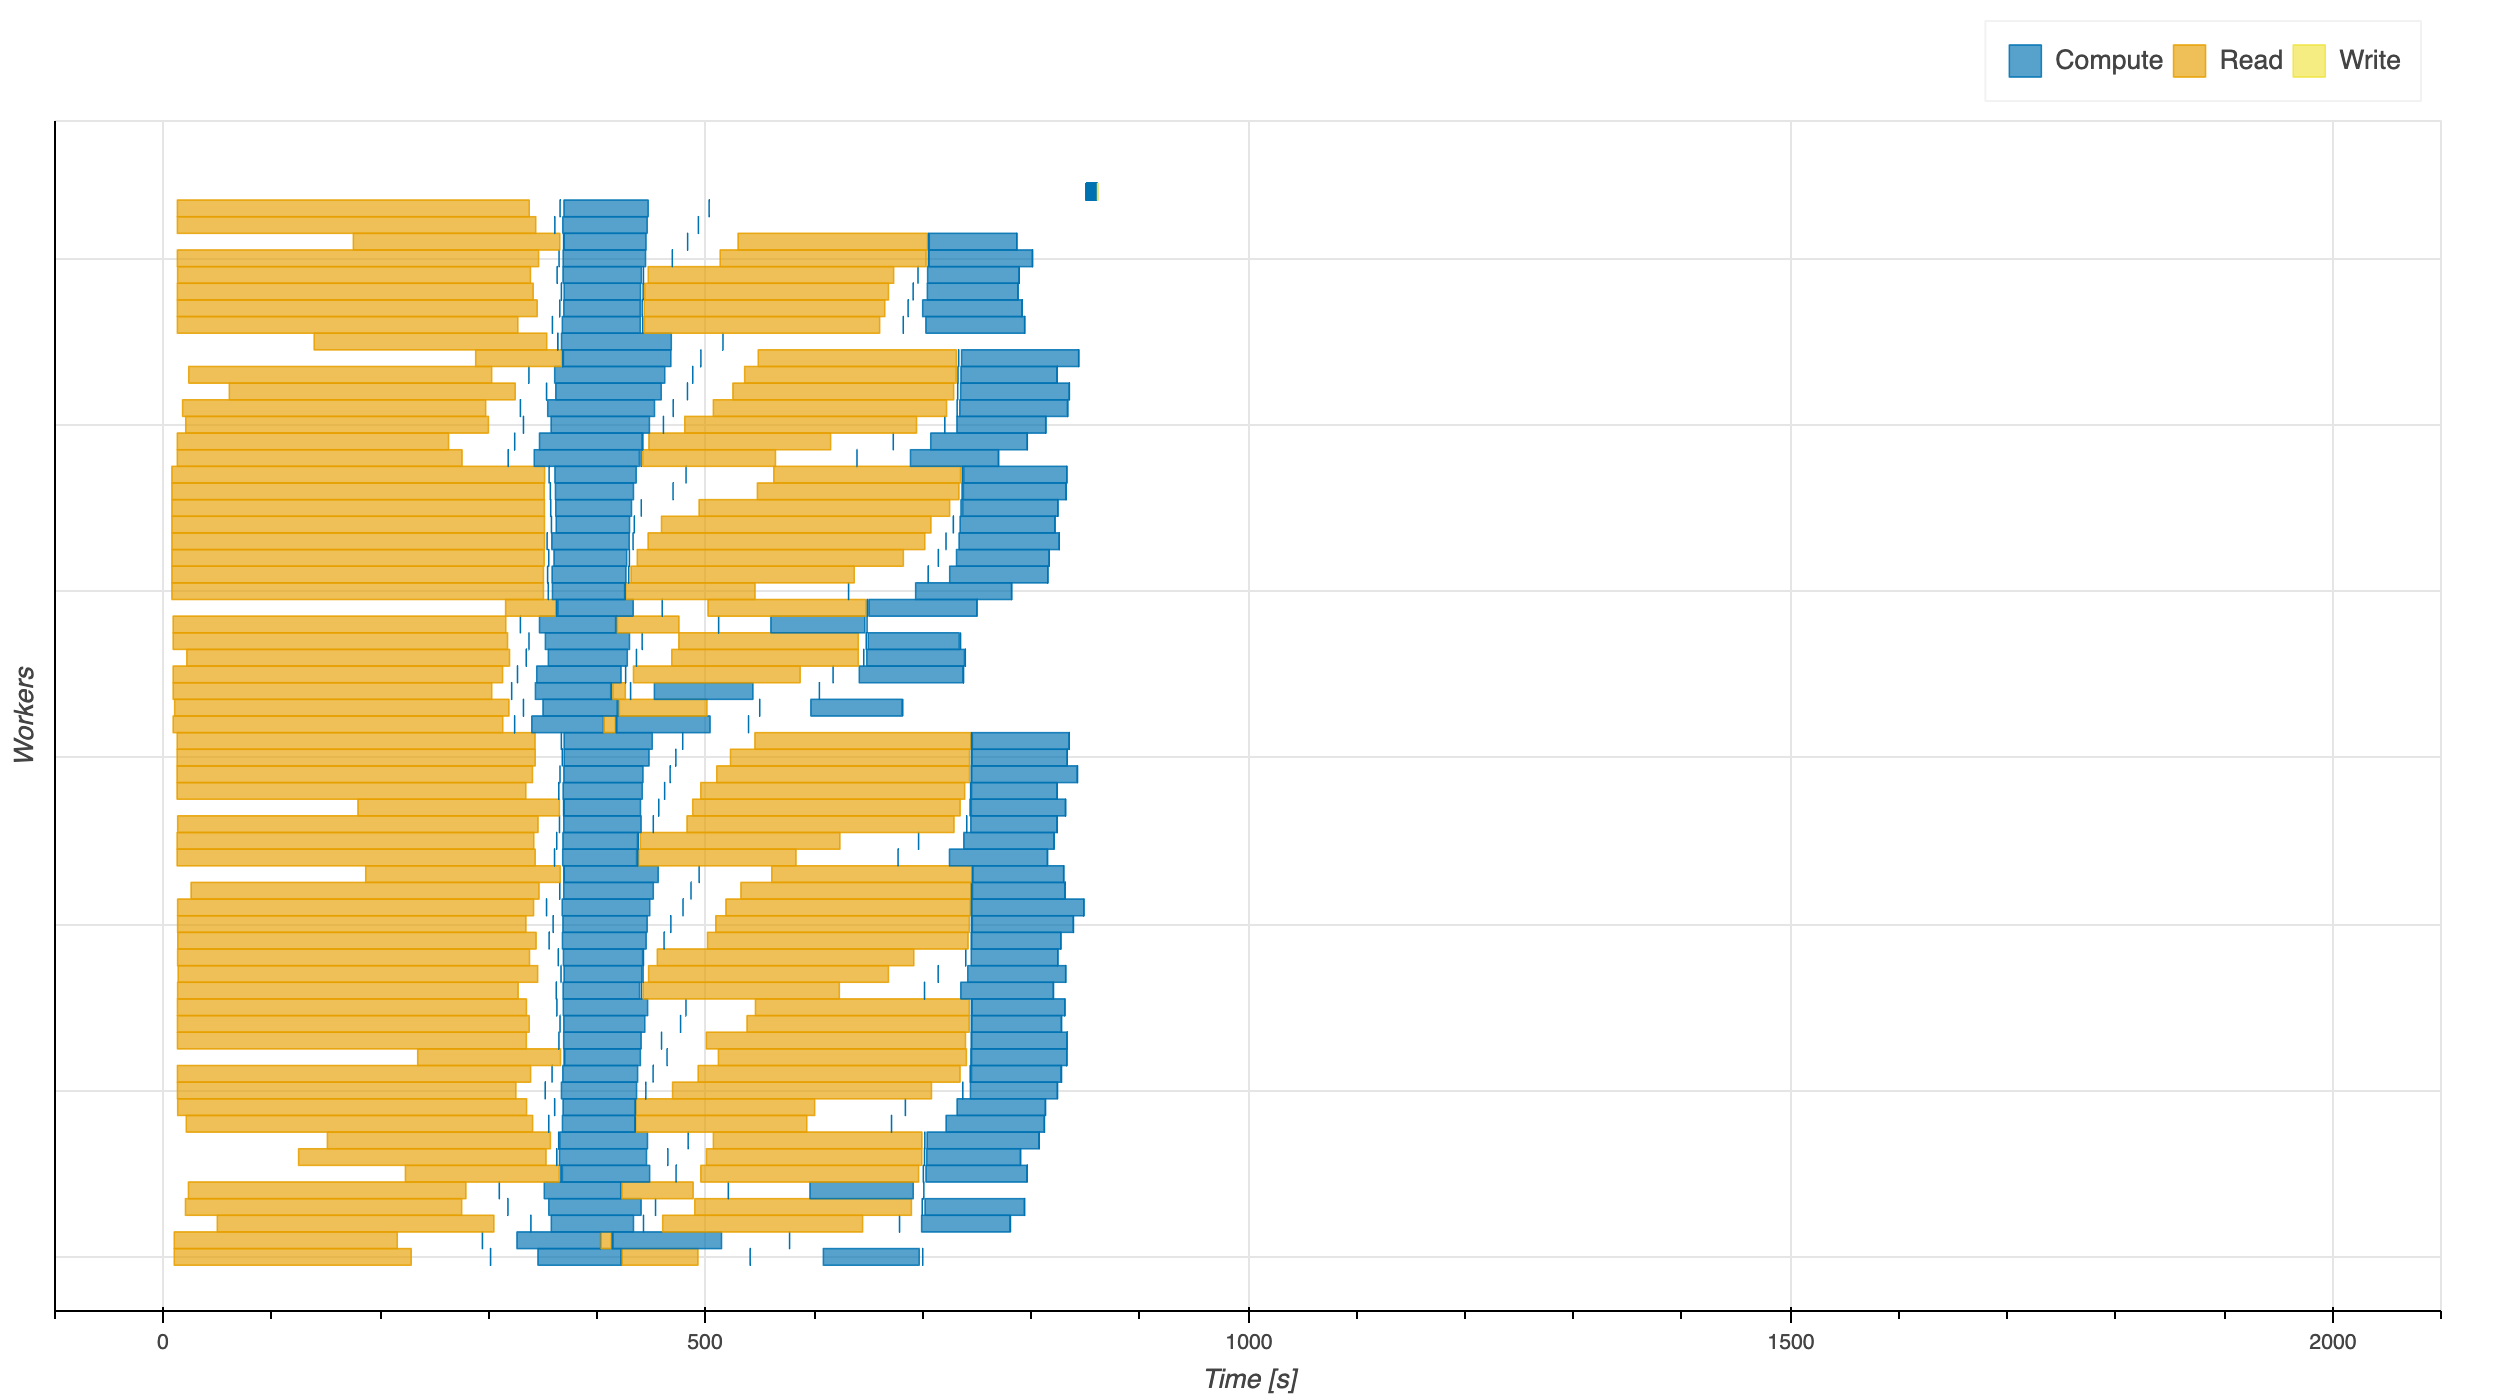
\includegraphics[clip,width=\columnwidth,
        height=0.15\textheight]{images/spark_histo_gantt.png}}
        \caption{Spark}\label{fig:histo_spark_gantt}
    \end{subfigure}
    \\
    \begin{subfigure}[b]{\columnwidth}
        \href{https://zenodo.org/record/3354434/files/dask-bag-histo-baseline.html?download=1}{
        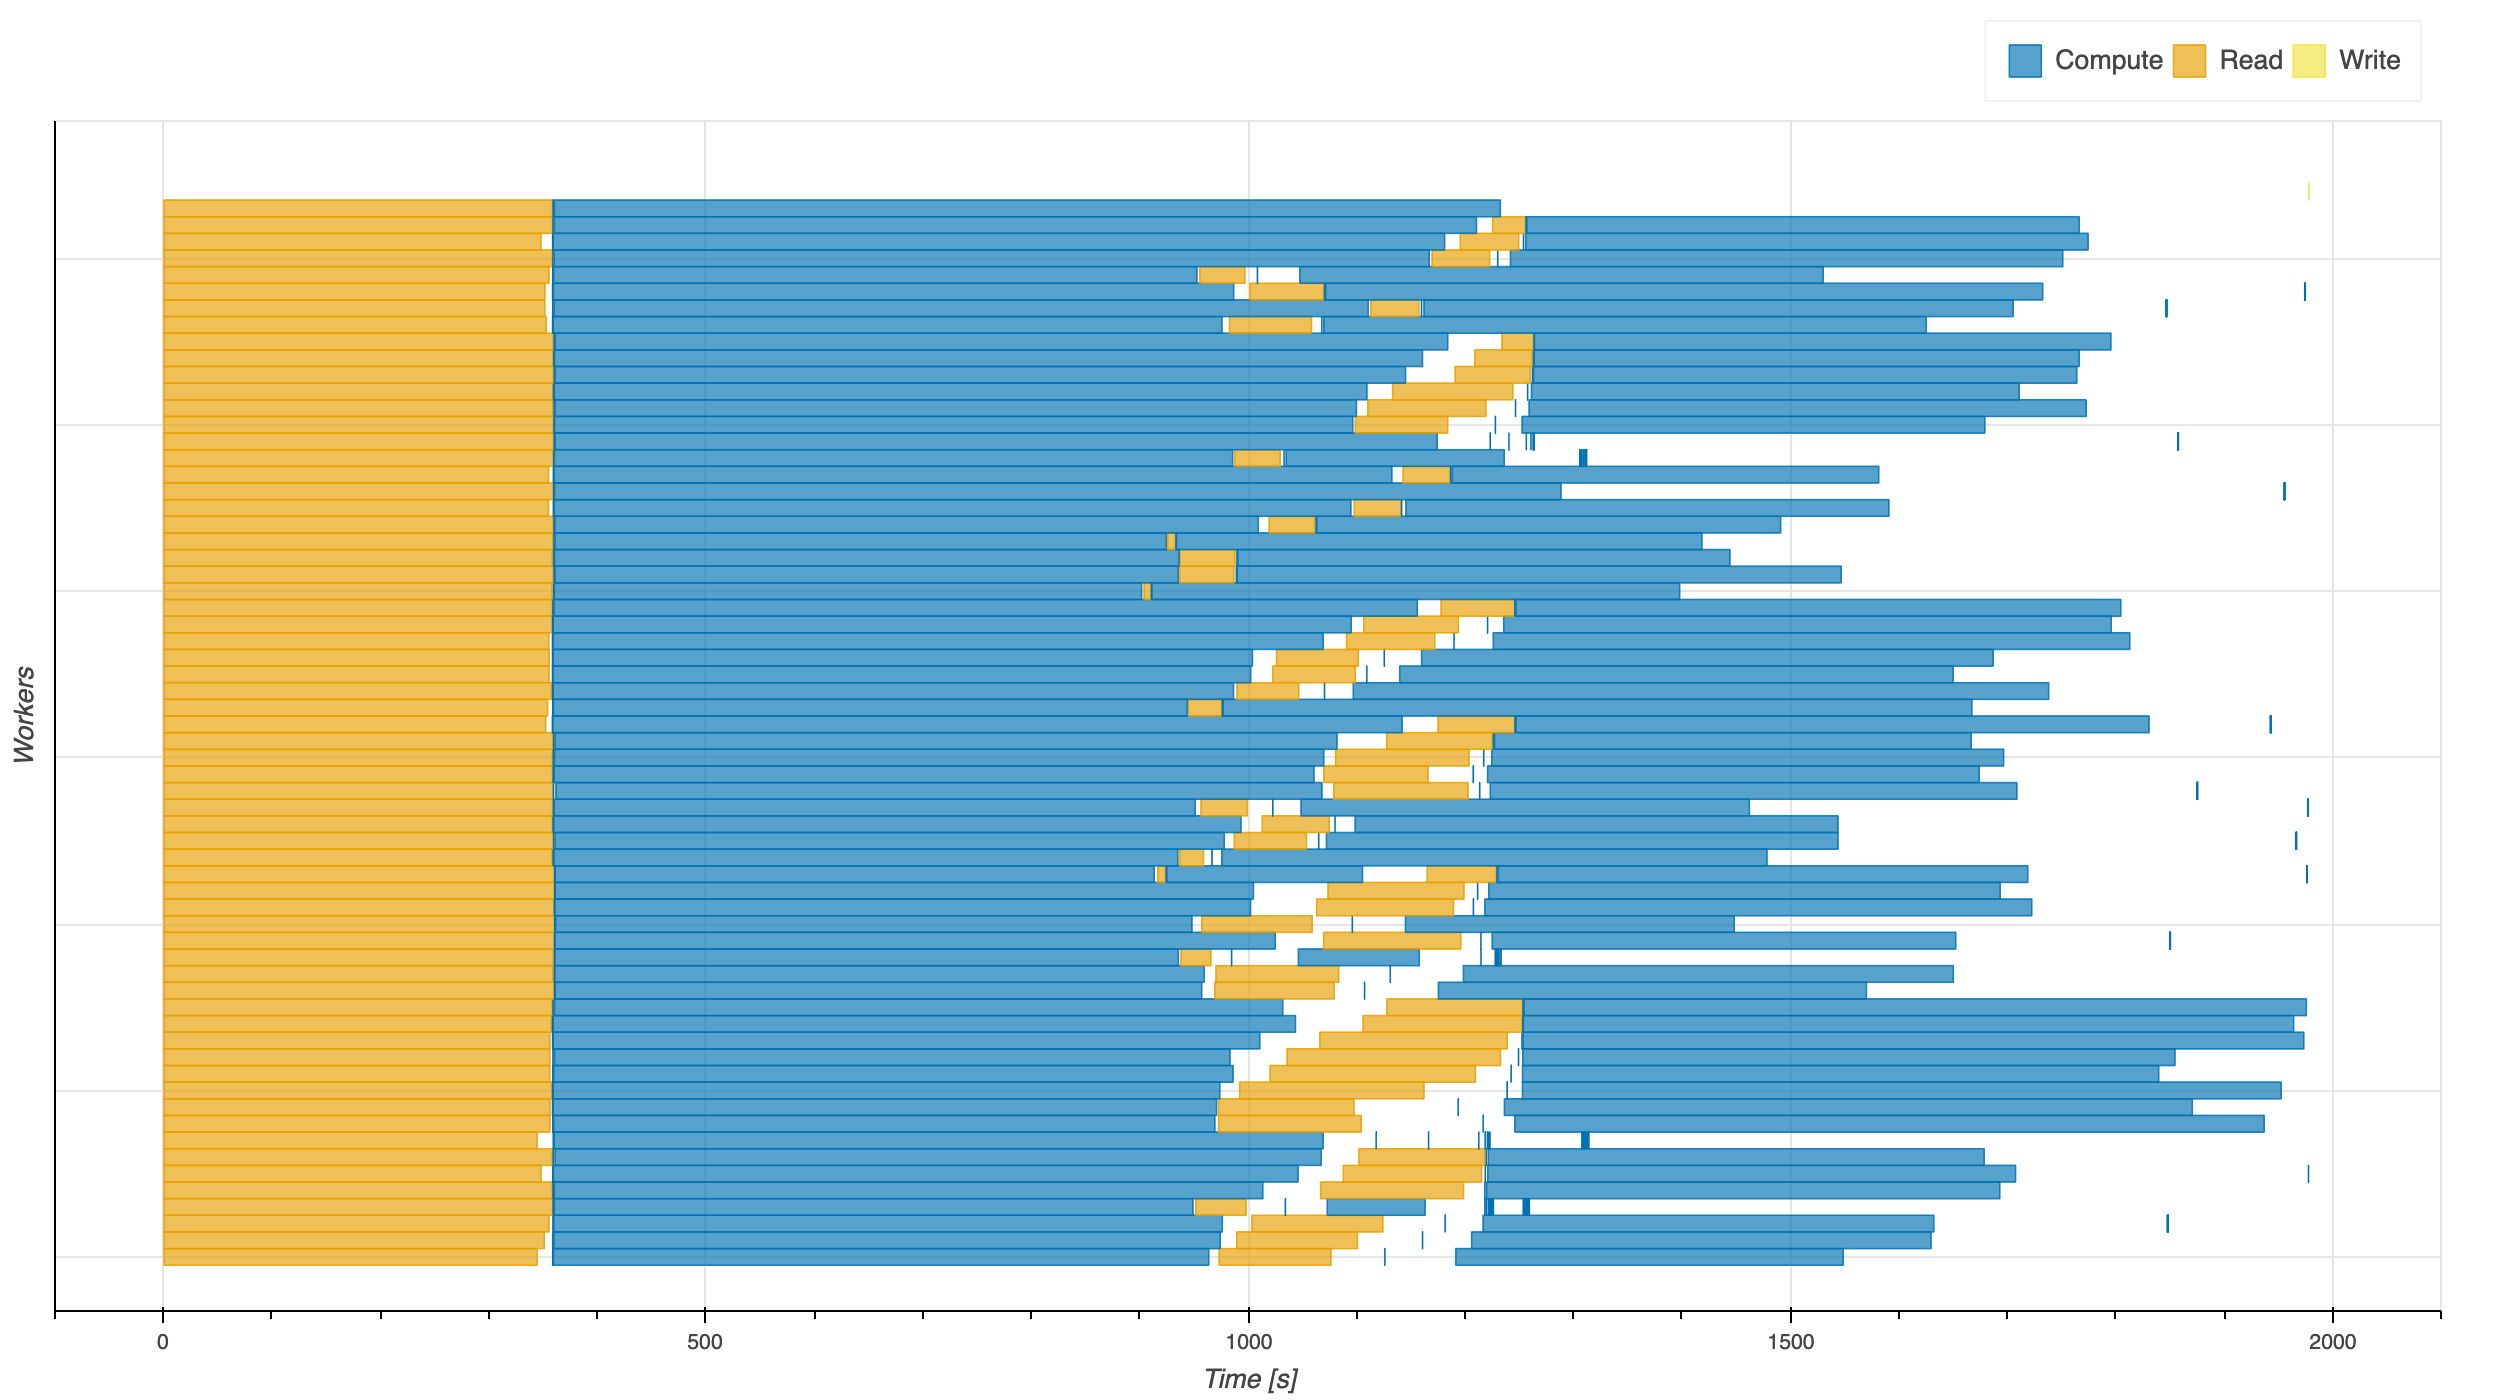
\includegraphics[clip,width=\columnwidth,
        height=0.15\textheight]{images/bag_histo_gantt.png}}
        \caption{Dask Bag}\label{fig:histo_dask_bag_gantt}
    \end{subfigure}
    \\
    \begin{subfigure}[b]{\columnwidth}
        \href{https://zenodo.org/record/3354434/files/dask-delayed-histo-baseline.html?download=1}{
        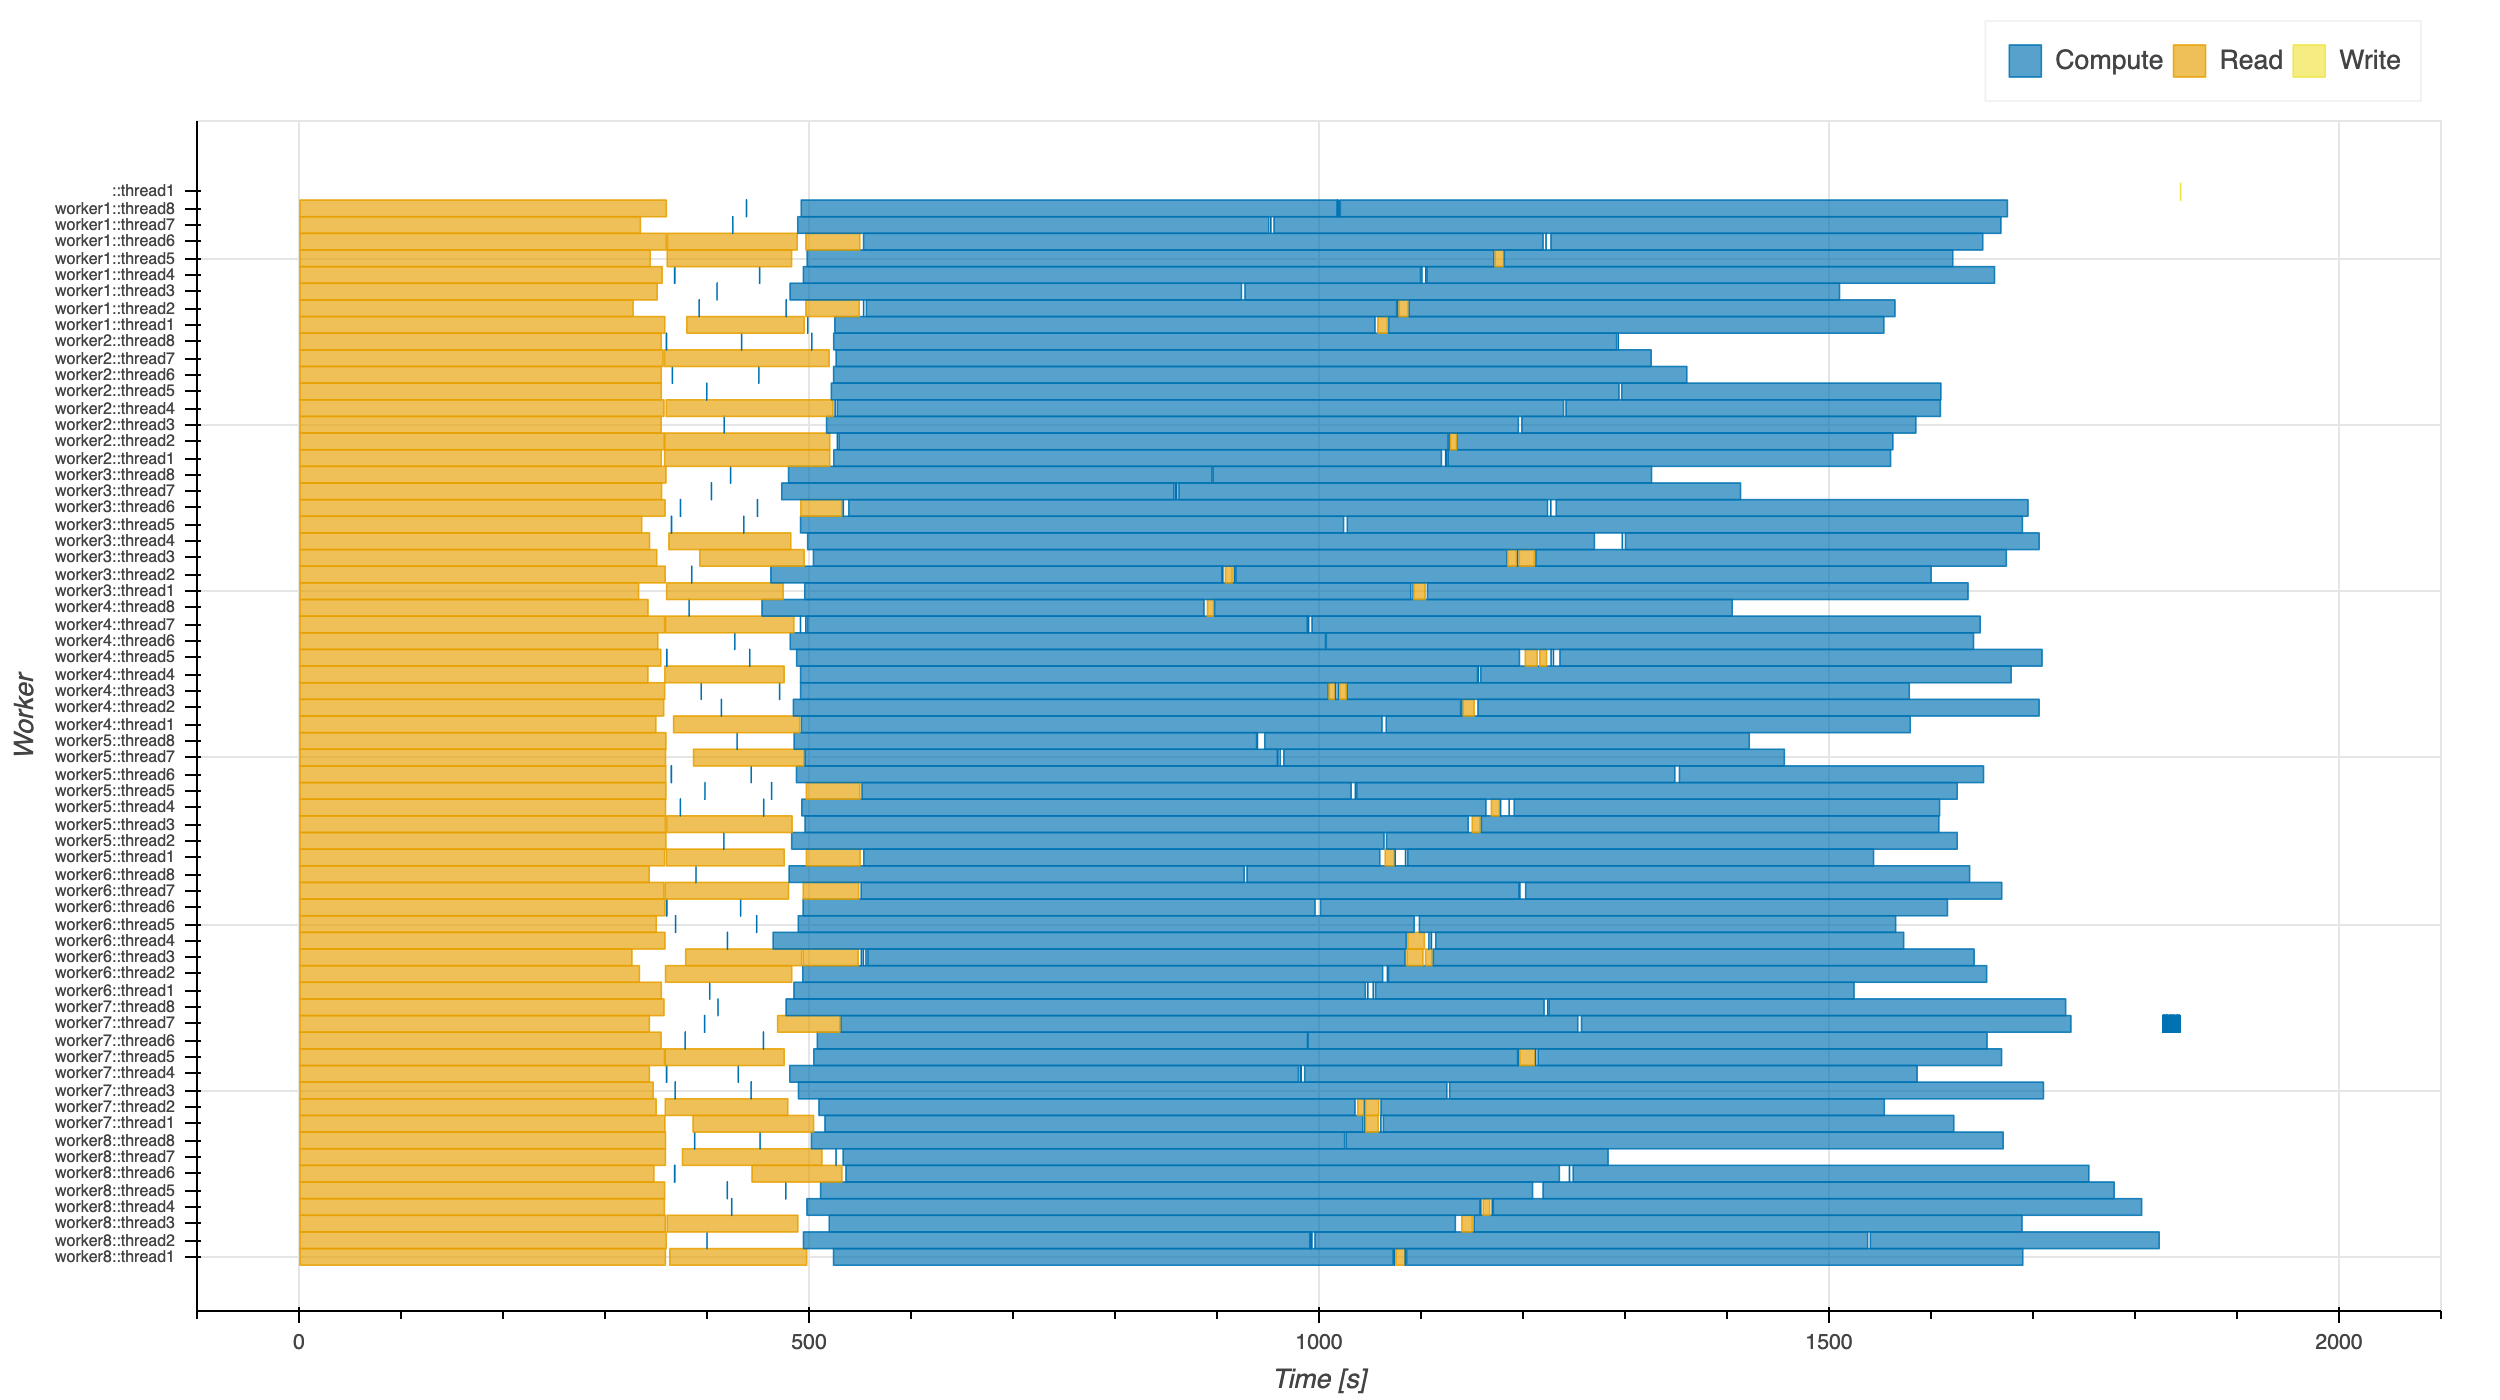
\includegraphics[clip,width=\columnwidth,
        height=0.15\textheight]{images/delayed_histo_gantt.png}}
        \caption{Dask Delayed}\label{fig:histo_dask_delayed_gantt}
    \end{subfigure}
    \caption{Histogram (Python): 125 blocks, 8 workers, 8
    CPUs/worker}\label{fig:histo_gantt}
\end{figure}

%%% HISTOGRAM (NumPy) %%%
\subsection{Histogram (NumPy): Number of workers}
Figure~\ref{fig:histo_np_ms_worker} shows the makespan for various amount of workers.
Overall, the makespan for all engines does not change considerably with an increase
in the number of workers. This is likely a result of using a non-distributed
shared file system. There is no
substantial difference between all engines although Delayed is slightly faster.
Figure~\ref{fig:histo_np_tt_worker} shows the total execution time
breakdown. The overhead and read time increase proportionally to the number
of workers thus increasing the total time. 

\begin{figure}[!b]
    \centering
    \begin{subfigure}[b]{\columnwidth}
        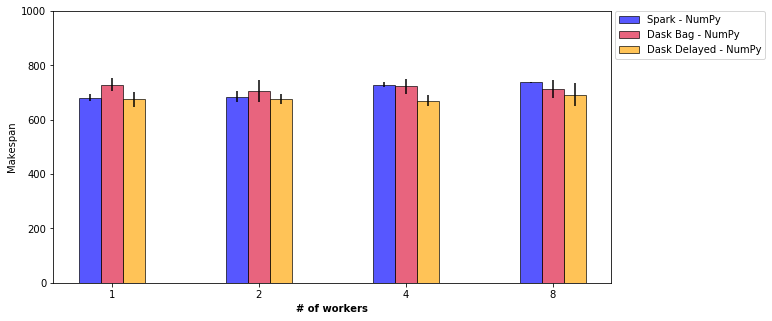
\includegraphics[clip,width=\columnwidth]{images/histo_np_worker.png}%
        \caption{Histogram (NumPy) makespan}\label{fig:histo_np_ms_worker}
    \end{subfigure}
    \\
    \begin{subfigure}[b]{\columnwidth}
        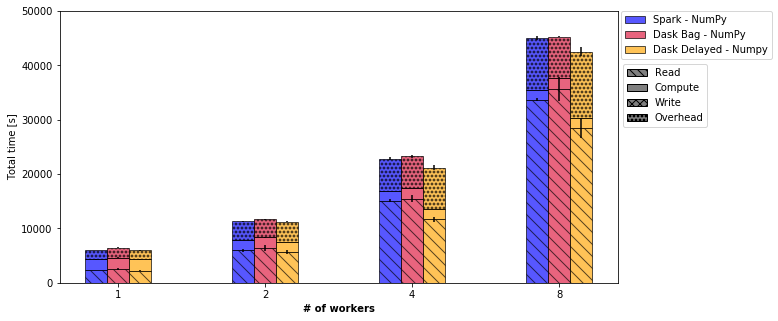
\includegraphics[clip,width=\columnwidth]{images/histo_idle_np_worker.png}%
        \caption{Histogram (NumPy) total time}\label{fig:histo_np_tt_worker}
    \end{subfigure}
    \caption{125 blocks, 8 CPUs/worker}
\end{figure}

\subsection{Histogram (NumPy): Number of blocks}
Figure~\ref{fig:histo_np_ms_block} shows the makespan of the application for
different block sizes. Overall, there is no substantial difference for
all engines and block sizes.

Figure~\ref{fig:histo_np_tt_block} shows the total time spent in each function.
Once more, since Delayed is thread-based its overhead at 30 blocks is seems much
higher that it really is. Considering the overhead error and that at 30 blocks
the workers only use half their core, the total time is substantially the same
for all block size. This is due to lower block sizes having a lower IO time,
however, it balances out by the resulting increase in overhead.

\begin{figure}[!t]
    \centering
    \begin{subfigure}[b]{\columnwidth}
        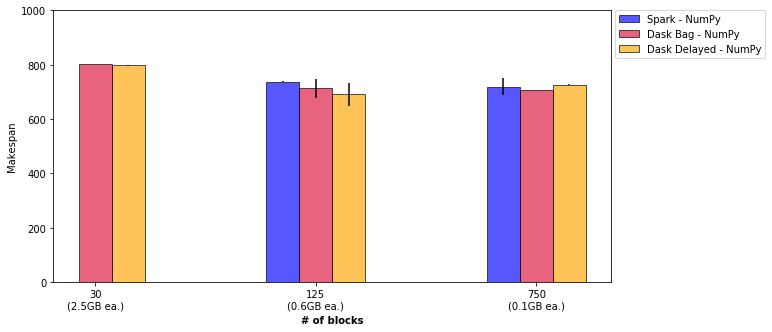
\includegraphics[clip,width=\columnwidth]{images/histo_np_block.png}%
        \caption{Histogram (NumPy) makespan}\label{fig:histo_np_ms_block}
    \end{subfigure}
    \\
    \begin{subfigure}[b]{\columnwidth}
        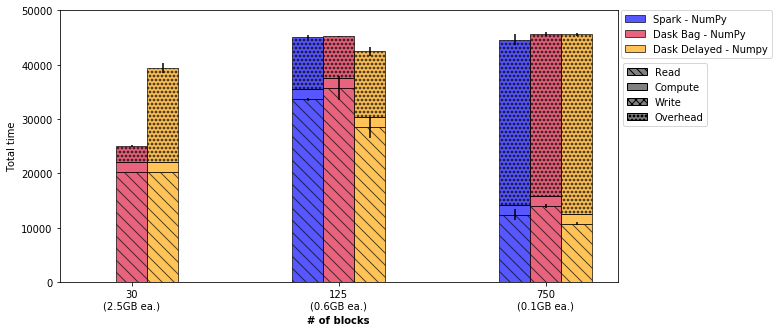
\includegraphics[clip,width=\columnwidth]{images/histo_idle_np_block.png}%
        \caption{Histogram (NumPy) total time}\label{fig:histo_np_tt_block}
    \end{subfigure}
    \caption{8 workers, 8 CPUs/worker}
\end{figure}

\subsection{Histogram (NumPy): Gantt chart}
Figure~\ref{fig:histo_np_gantt} shows the Gantt chart of the baseline for the
Histogram (NumPy) experiment. The overhead for Spark and Bag is mostly located
between read and compute tasks. On the other hand, Delayed
overhead is dispersed between all types of tasks. This causes Delayed to
overlap more compute and read tasks simultaneously amongst different workers.

In Figure~\ref{fig:histo_np_gantt}, read tasks are initially similar for all
engines. However, when computation starts the subsequent read tasks are much
shorter for Delayed. This is due the desynchronization of the task reducing the
IO bottleneck.



\begin{figure}[!tb]
    \centering
    \begin{subfigure}[b]{\columnwidth}
        \href{https://zenodo.org/record/3354434/files/spark-histo_np-baseline.html?download=1}{
        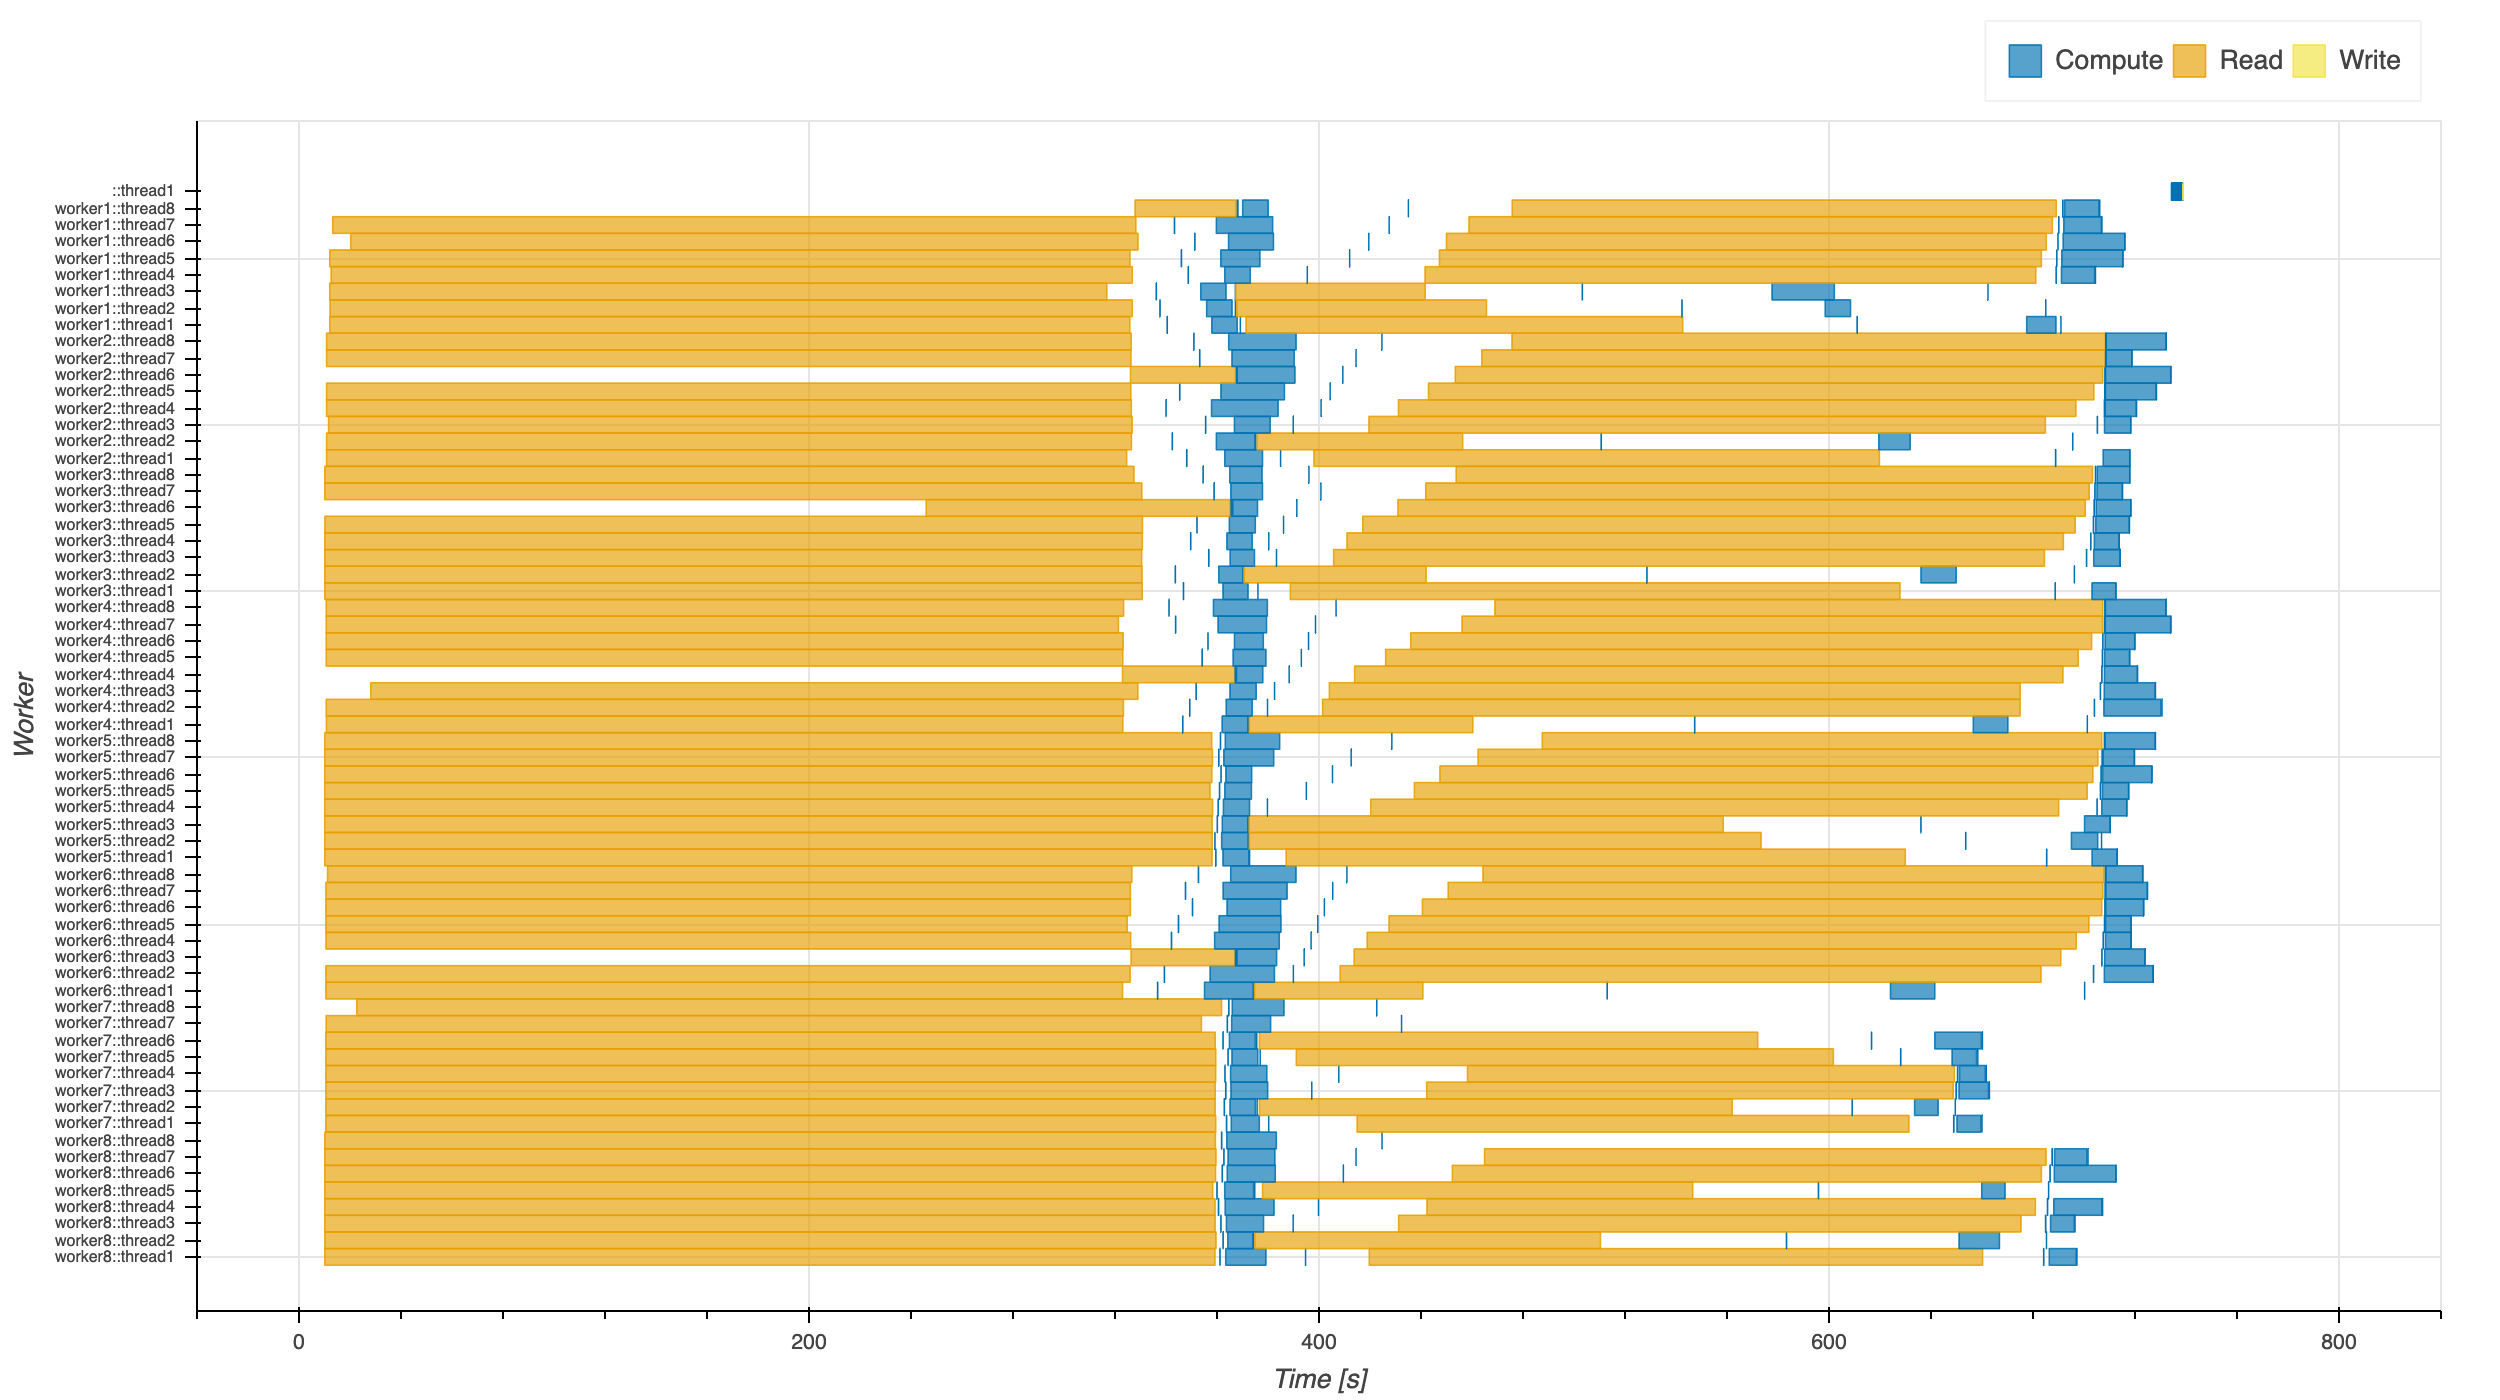
\includegraphics[clip,width=\columnwidth,
        height=0.15\textheight]{images/spark_histo_np_gantt.png}}
        \caption{Spark}\label{fig:histo_np_spark_gantt}
    \end{subfigure}
    \\
    \begin{subfigure}[b]{\columnwidth}
        \href{https://zenodo.org/record/3354434/files/dask-bag-histo_np-baseline.html?download=1}{
        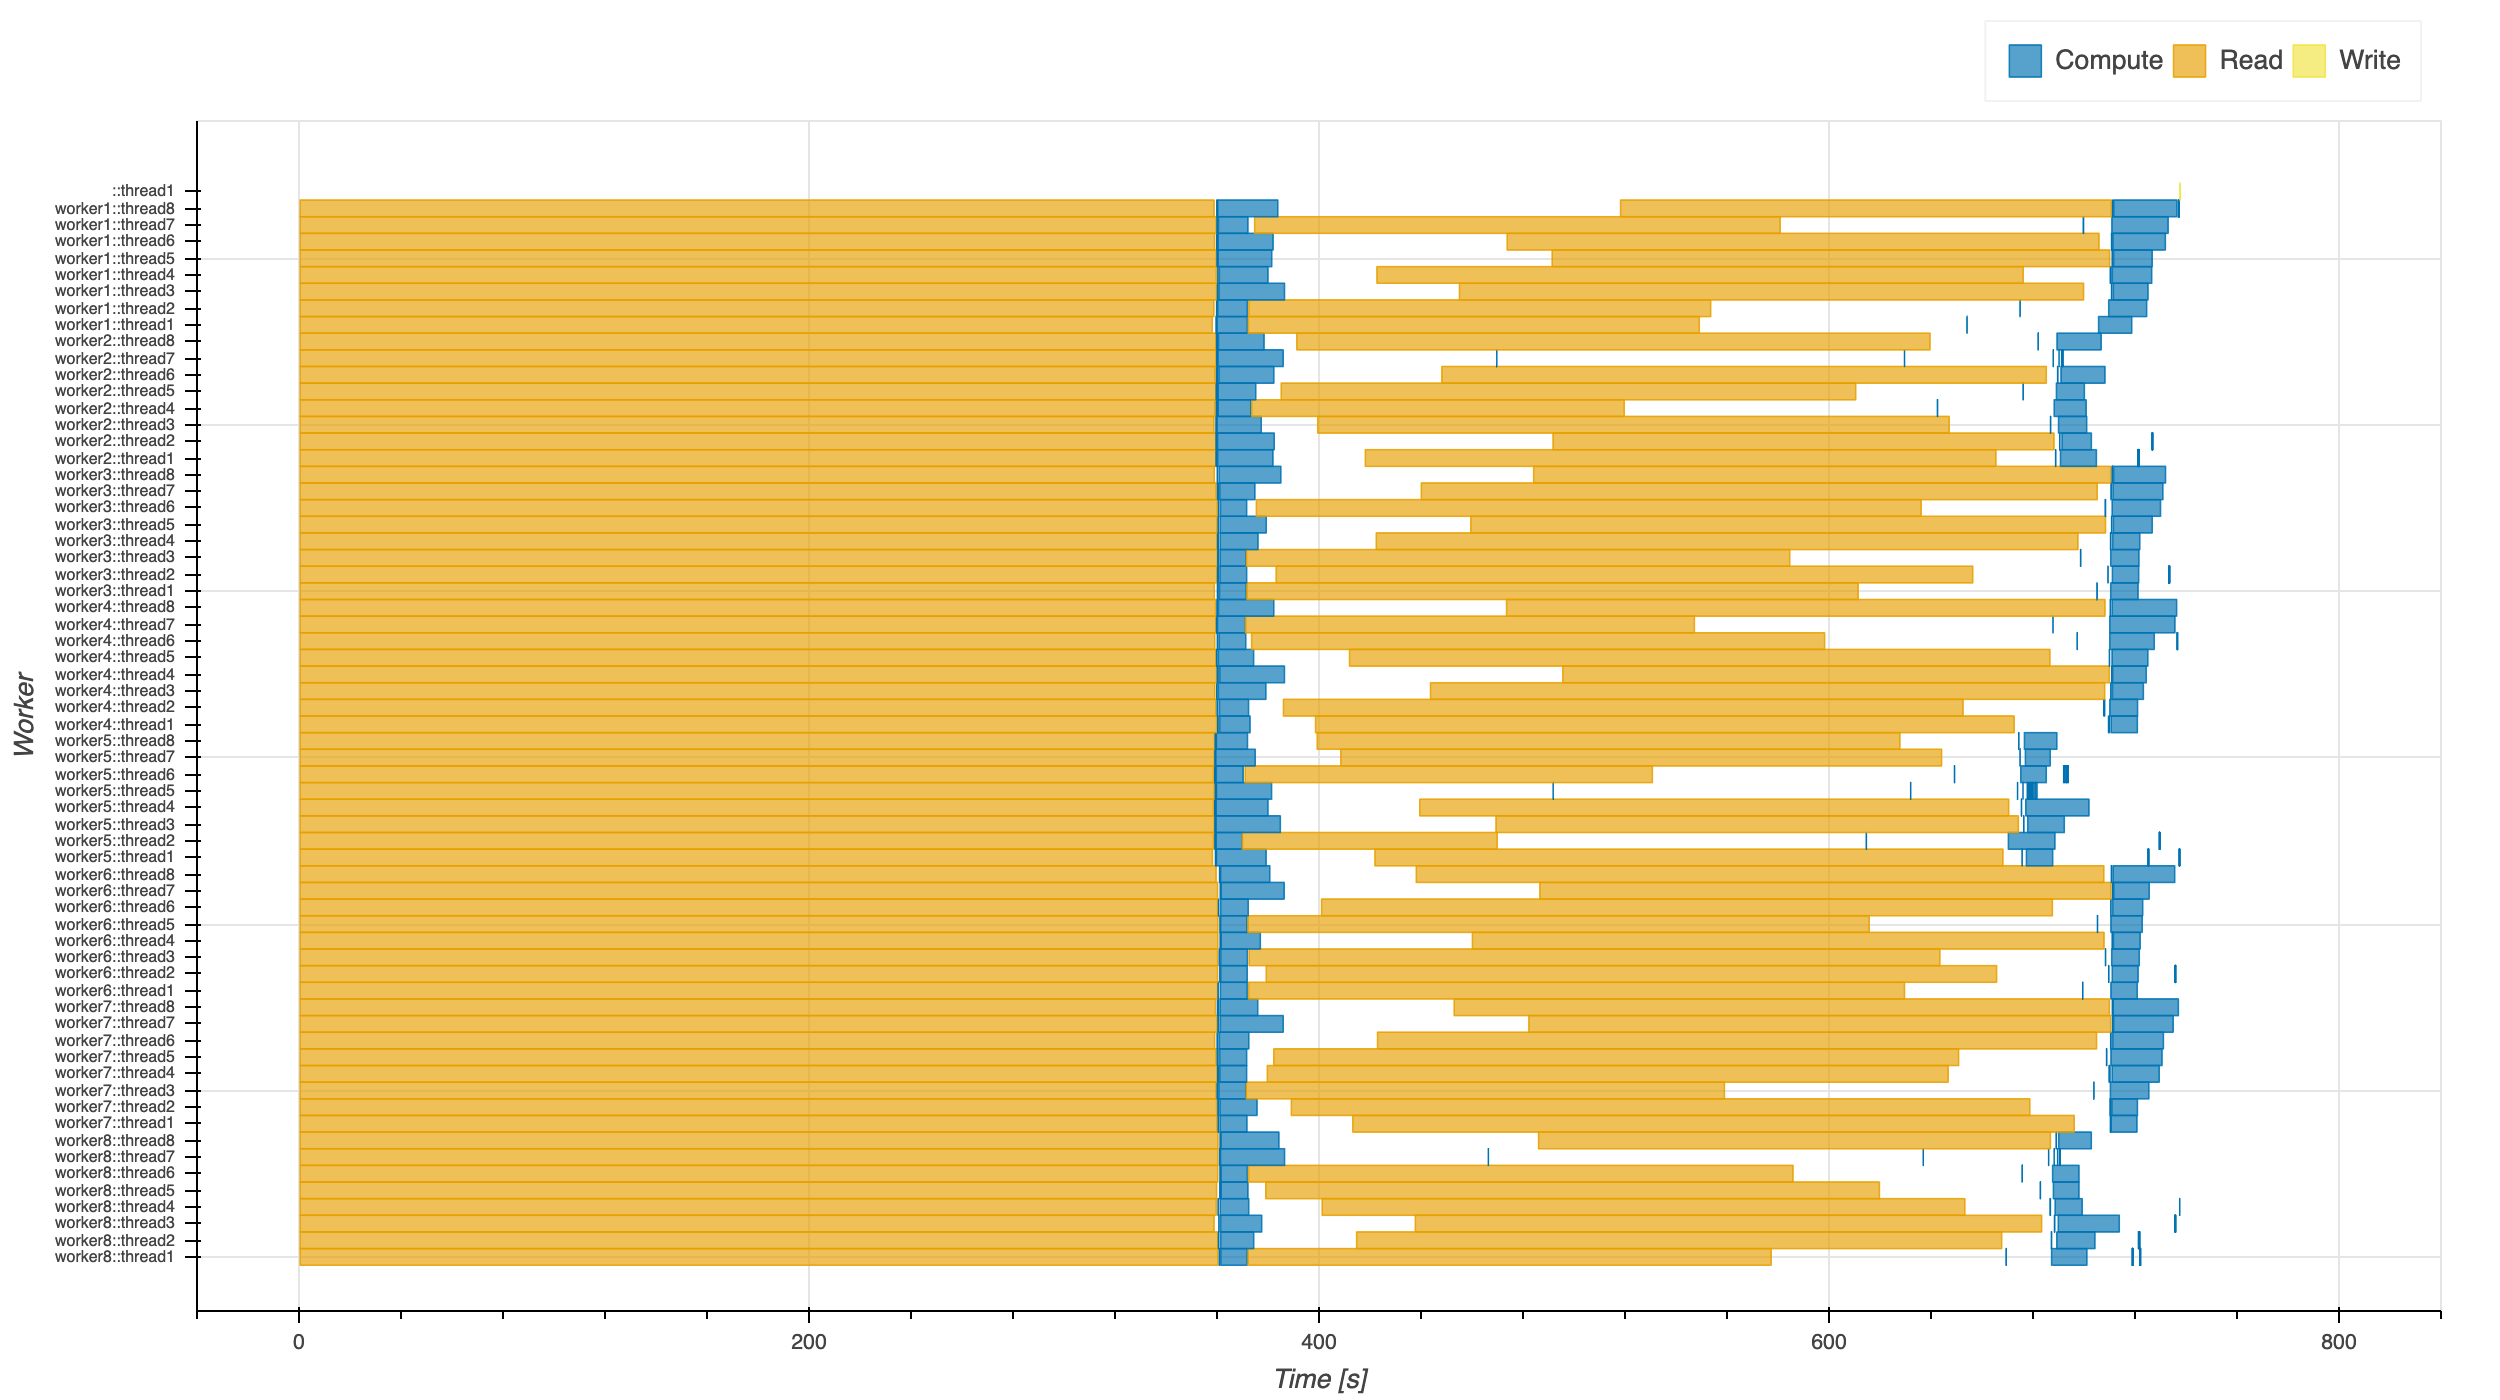
\includegraphics[clip,width=\columnwidth,
        height=0.15\textheight]{images/bag_histo_np_gantt.png}}
        \caption{Dask Bag}\label{fig:histo_np_dask_bag_gantt}
    \end{subfigure}
    \\
    \begin{subfigure}[b]{\columnwidth}
        \href{https://zenodo.org/record/3354434/files/dask-delayed-histo_np-baseline.html?download=1}{
        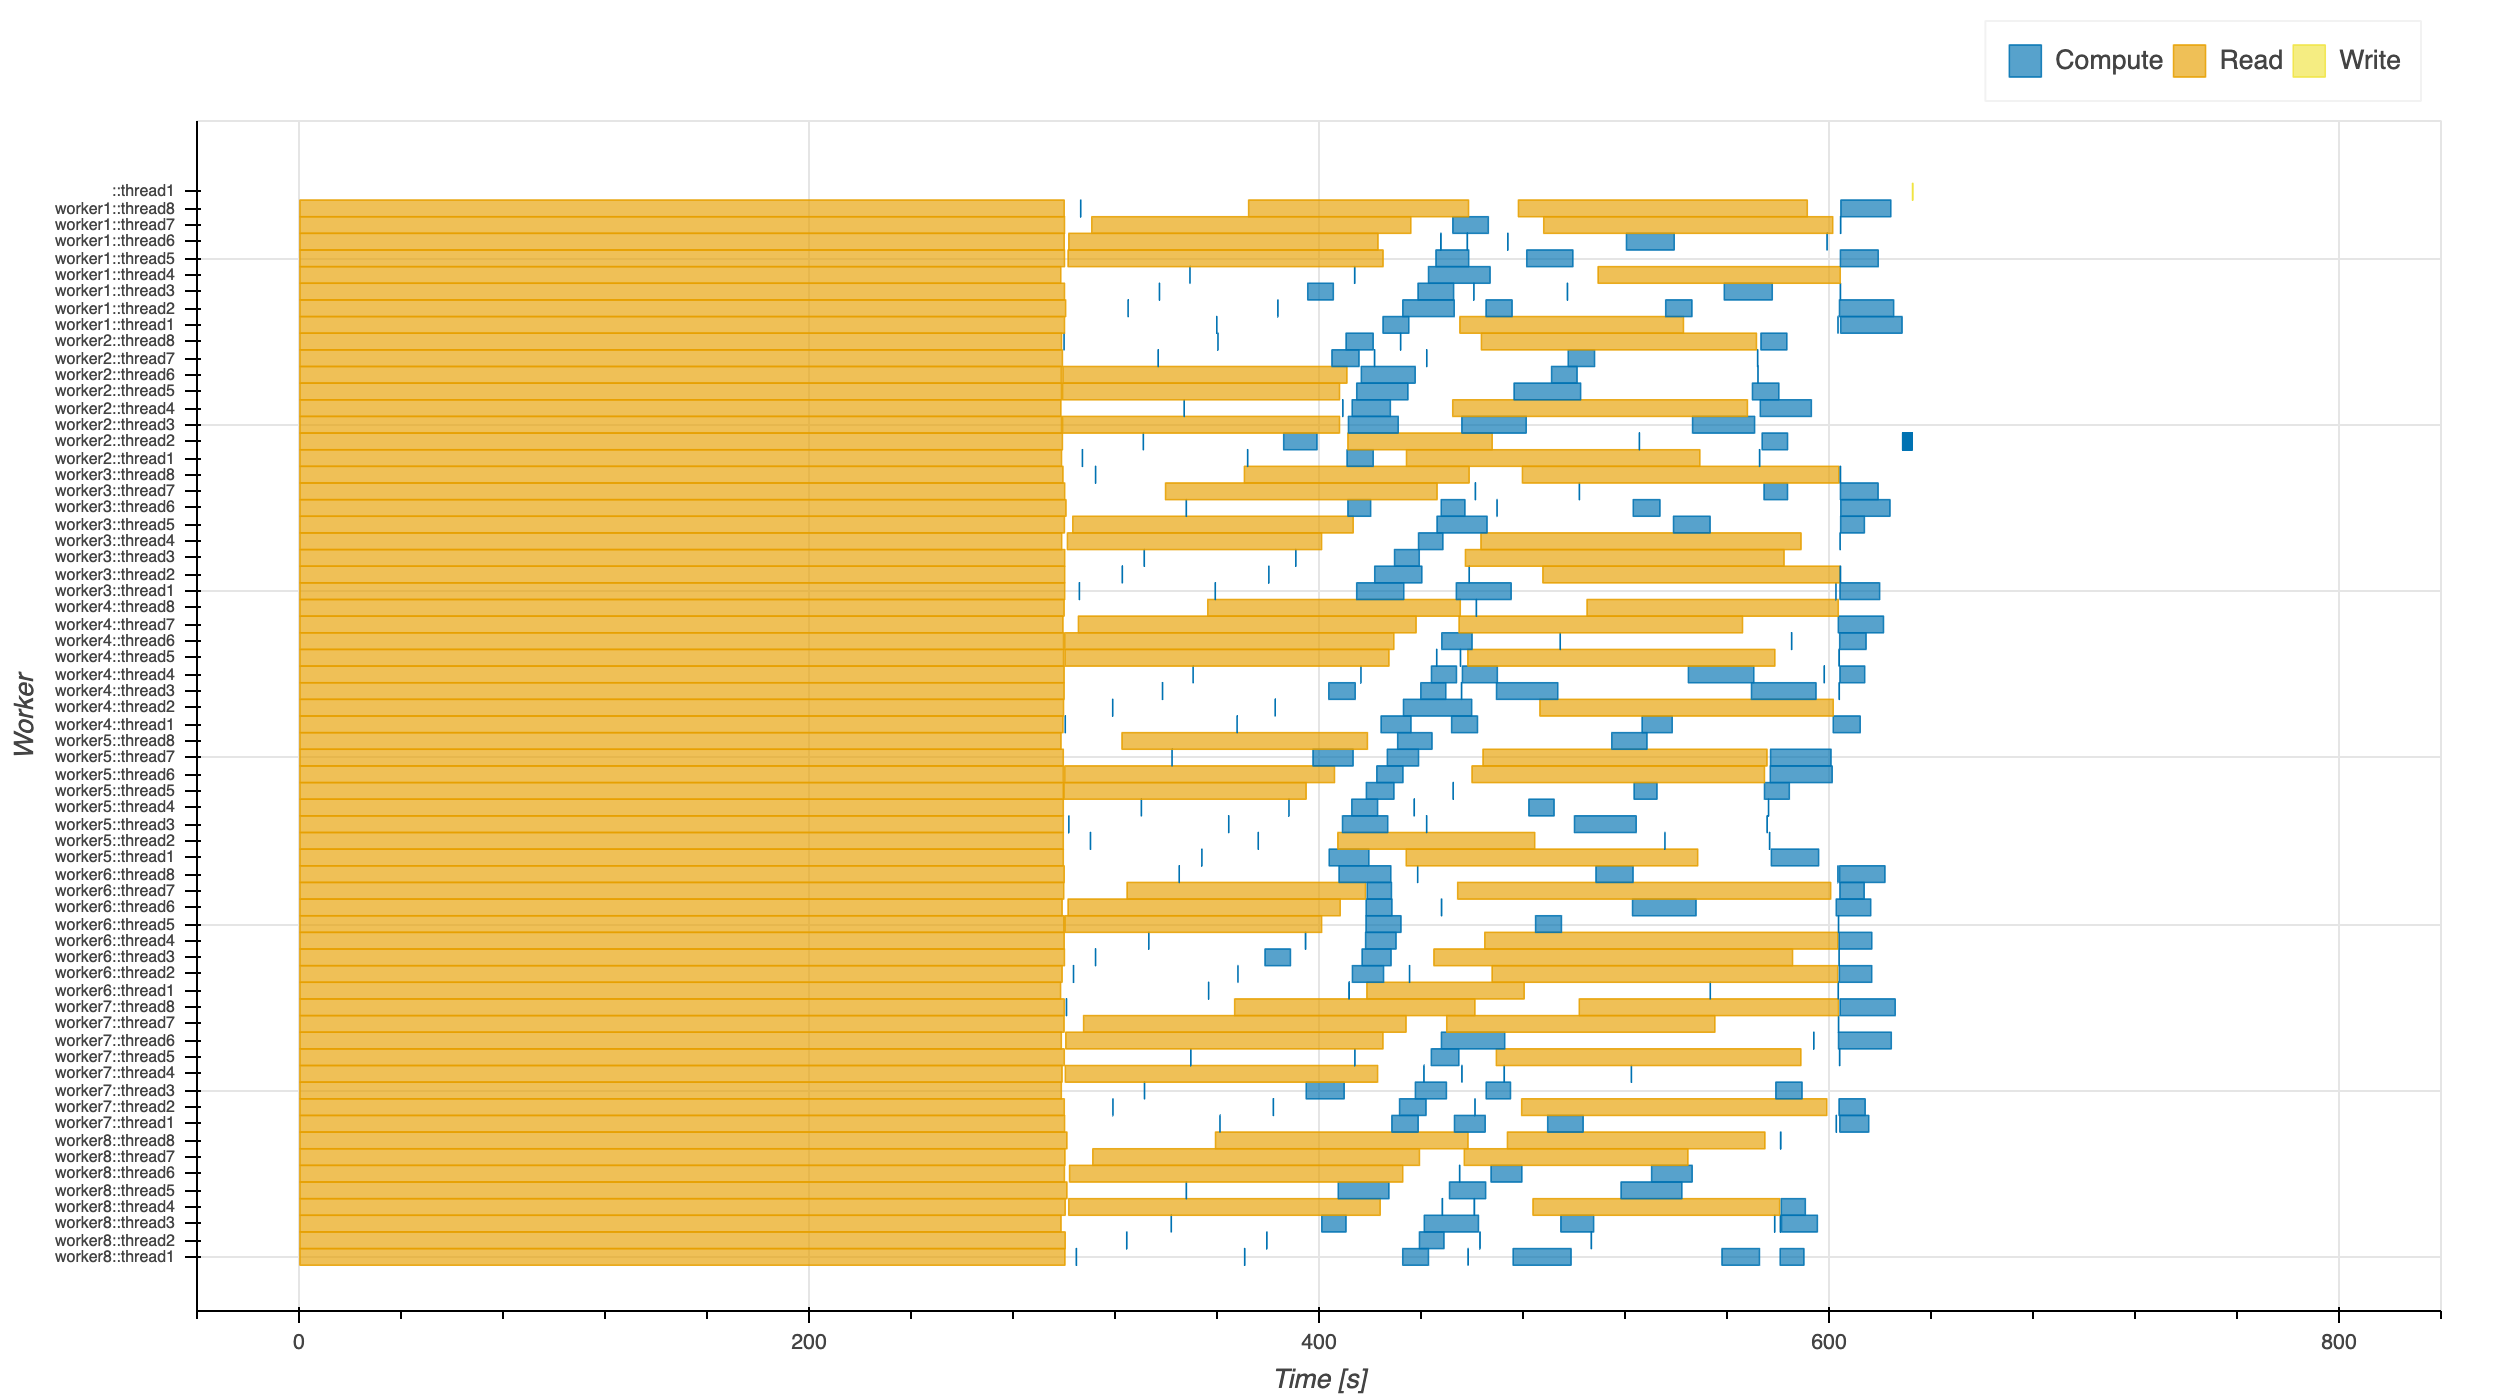
\includegraphics[clip,width=\columnwidth,
        height=0.15\textheight]{images/delayed_histo_np_gantt.png}}
        \caption{Dask Delayed}\label{fig:histo_np_dask_delayed_gantt}
    \end{subfigure}
    \caption{Histogram (NumPy): 125 blocks, 8 workers, 8
    CPUs/worker}\label{fig:histo_np_gantt}
\end{figure}

%%% BIDS EXAMPLE %%%
\subsection{BidsApp example: Number of workers}
Figure~\ref{fig:bids_ms_worker} shows the makespan of the application when
varying the amount of workers. Overall, there is no substantial difference
between the engines. The makespan scales well with the increase in workers,
however, the scaling reduces slightly when reaching 8 workers. This is due
to an increase in I/O time caused by parallel accesses to 
the shared file system.

In Figure~\ref{fig:bids_tt_worker}, the total execution time of each function is
shown. Each engine has a similar total time independently of its number of workers.
Consistently with previous observations, the overhead increases substantially with the 
number of workers.

% The overhead increases
% proportionally with the number of workers (see regression lines below). This is due
% to more communication between the scheduler and workers as well as intra-worker and
% inter-worker communication.


% \hspace{1cm}\(\hat{y}=223.53586\cdot{x} + 91.616964\) (Spark)

% \hspace{1cm}\(\hat{y}=182.82659\cdot{x} - 11.43834\) (Bag)

% \hspace{1cm}\(\hat{y}=172.54183\cdot + 400.69433\) (Delayed)

% \hspace{1cm}\(\hat{y}=132.41481\cdot{x} + 90.32813\) (Futures)

\begin{figure}[!t]
    \centering
    \begin{subfigure}[b]{\columnwidth}
        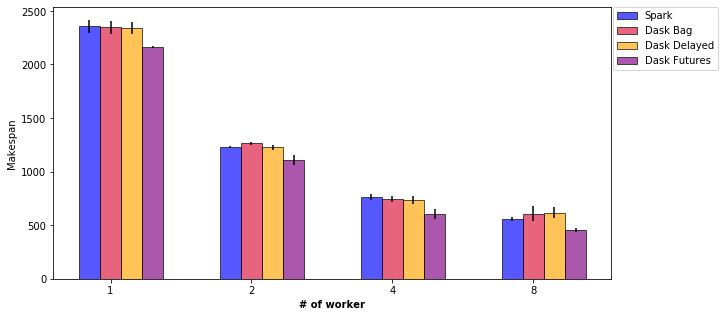
\includegraphics[clip,width=\columnwidth]{images/bids_worker.png}%
        \caption{BIDS App example makespan}\label{fig:bids_ms_worker}
    \end{subfigure}
    \\
    \begin{subfigure}[b]{\columnwidth}
        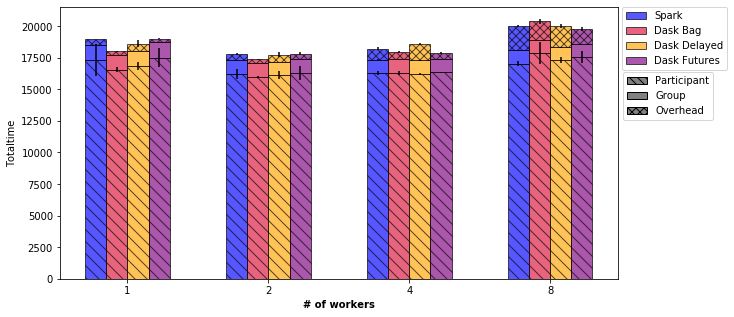
\includegraphics[clip,width=\columnwidth]{images/bids_idle_worker.png}%
        \caption{BIDS App example total time}\label{fig:bids_tt_worker}
    \end{subfigure}
    \caption{Variation of the amount of worker, 8 CPUs/worker}
\end{figure}


%% Baseline gantt chart
\subsection{BidsApp example: Gantt chart}
Figure~\ref{fig:bids_gantt} shows the Gantt chart obtained for each engine.
Gantt charts are structured in two parts: participant analysis (orange) and
group analysis (blue). The participant analysis tasks differ greatly in length. This
is due to the unequal amount of sessions per subject processed. The group analysis
is similar for all engines and APIs. Overall, most of the overhead encountered
results from the transition between the two analysis. This is because the group
analysis requires the results of the participant analysis to start.

\begin{figure}[!htb]
    \centering
    \begin{subfigure}[b]{\columnwidth}
        \href{https://zenodo.org/record/3354434/files/spark-bids-baseline.html?download=1}{
        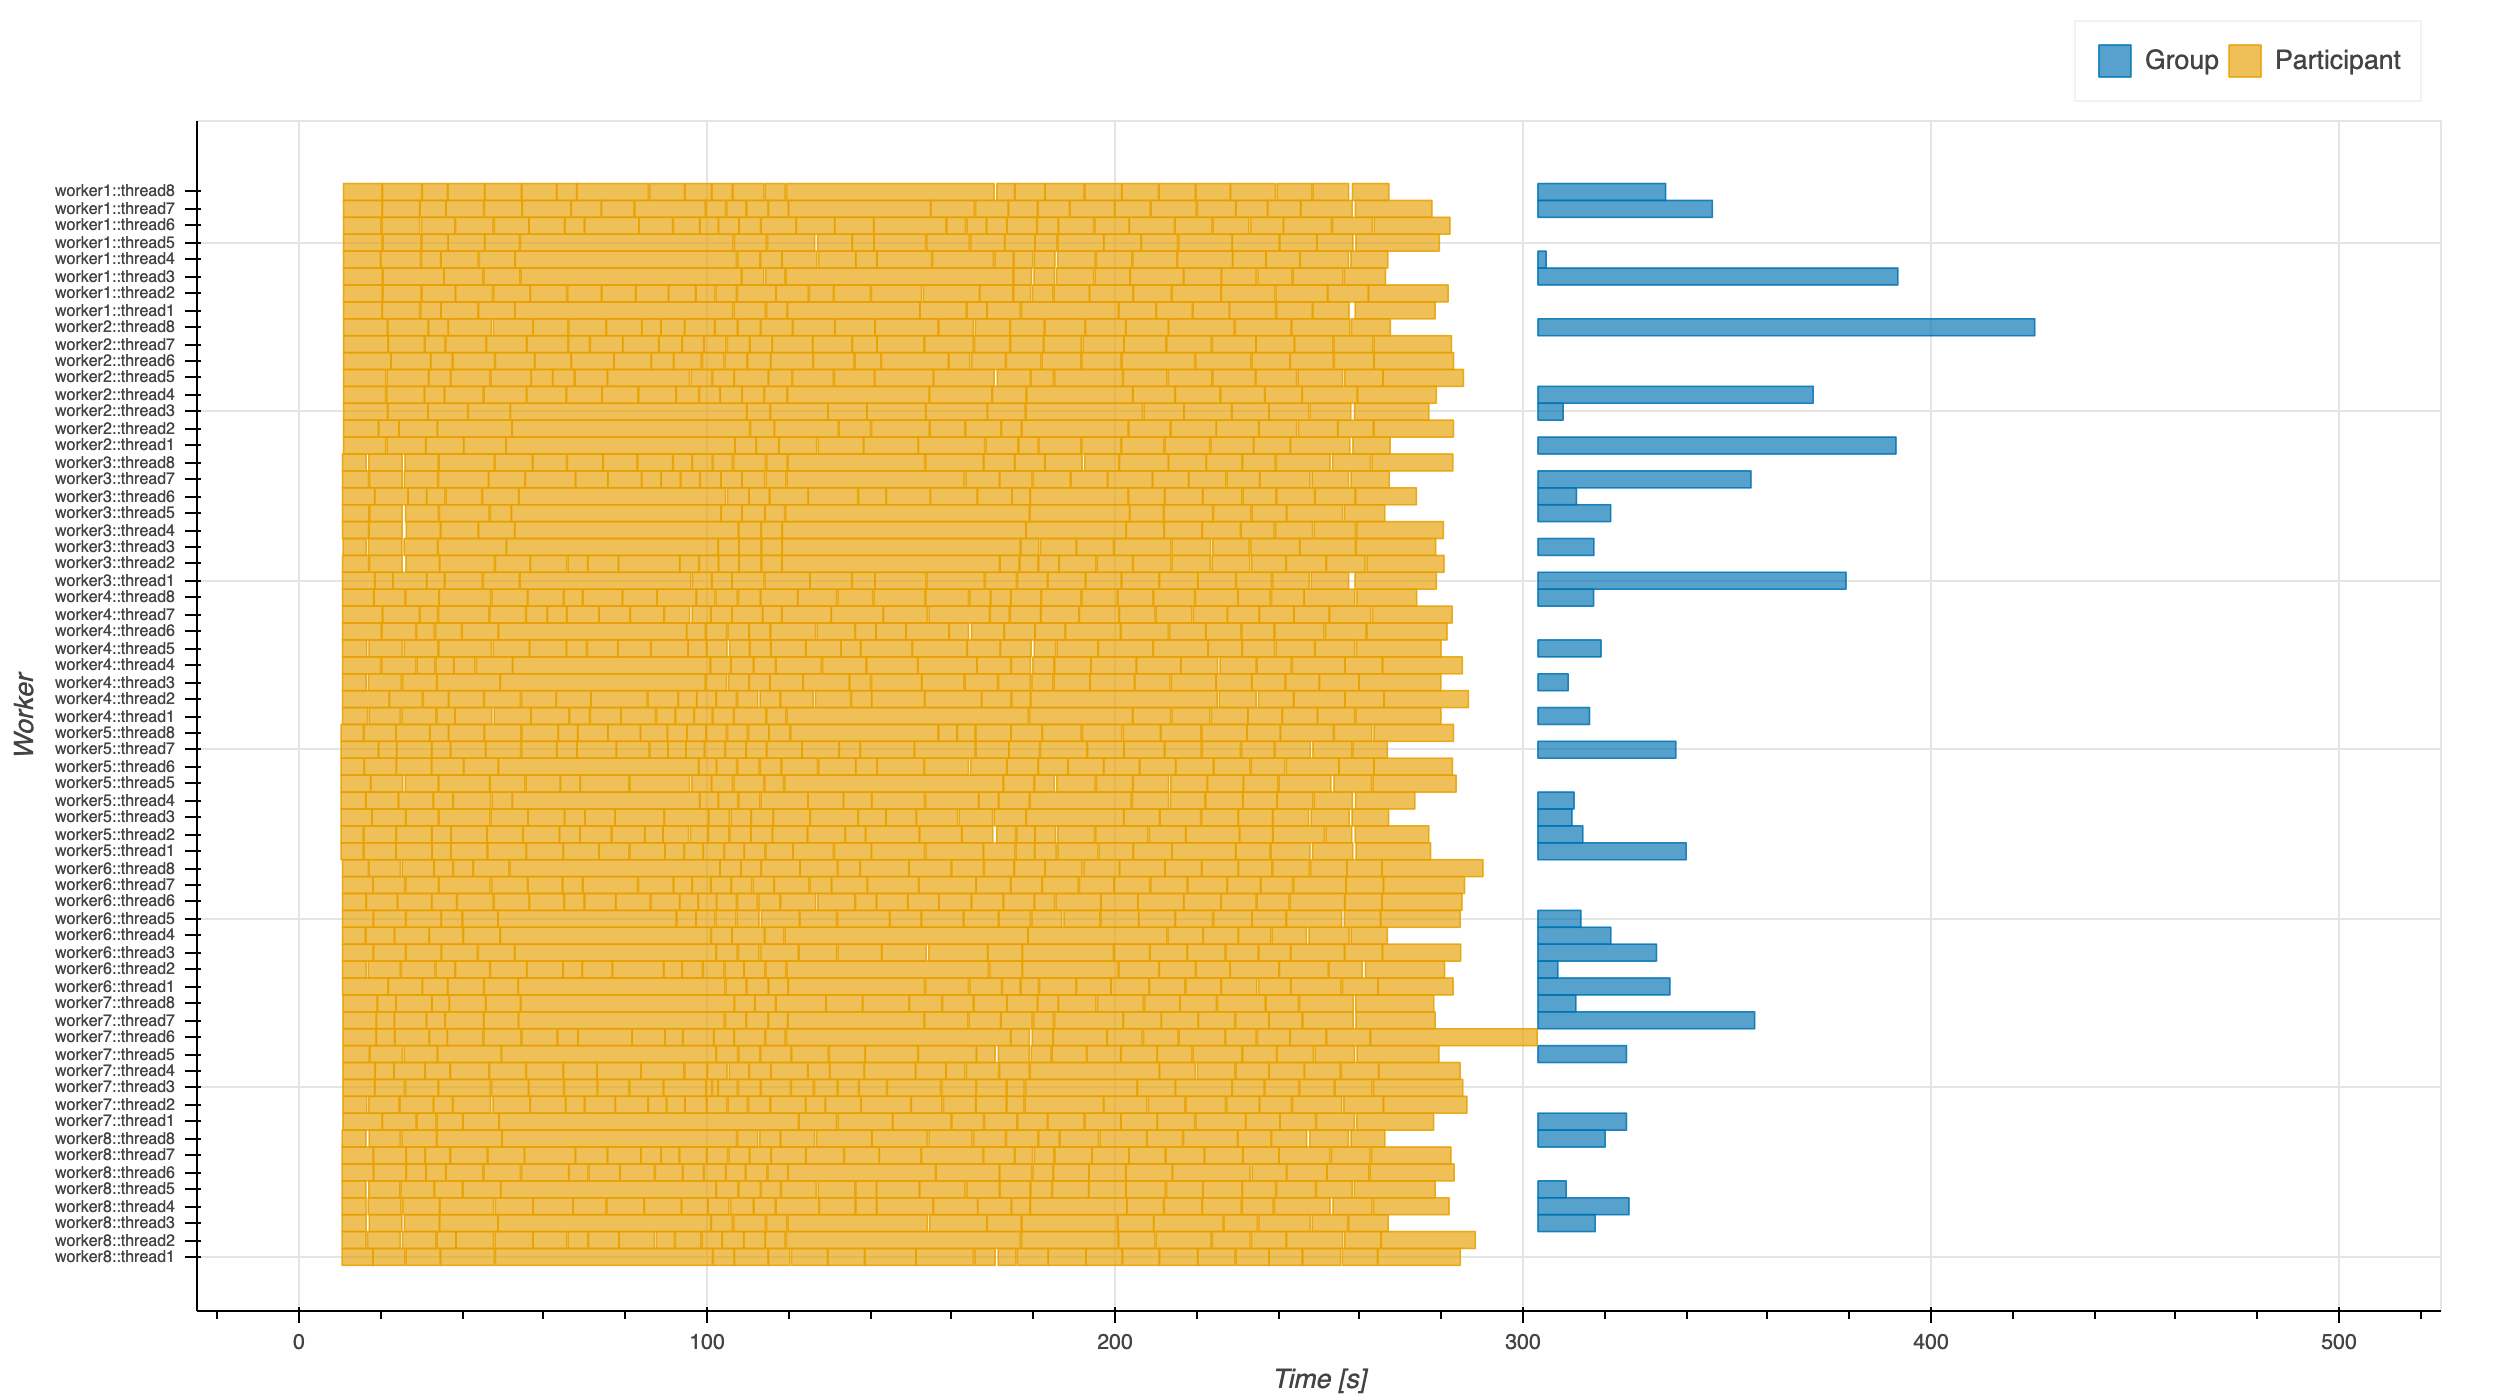
\includegraphics[clip,width=\columnwidth,
        height=0.15\textheight]{images/spark_bids_gantt.png}}
        \caption{Spark}\label{fig:bids_spark_gantt}
    \end{subfigure}
    \\
    \begin{subfigure}[b]{\columnwidth}
        \href{https://zenodo.org/record/3354434/files/dask-bag-bids-baseline.html?download=1}{
        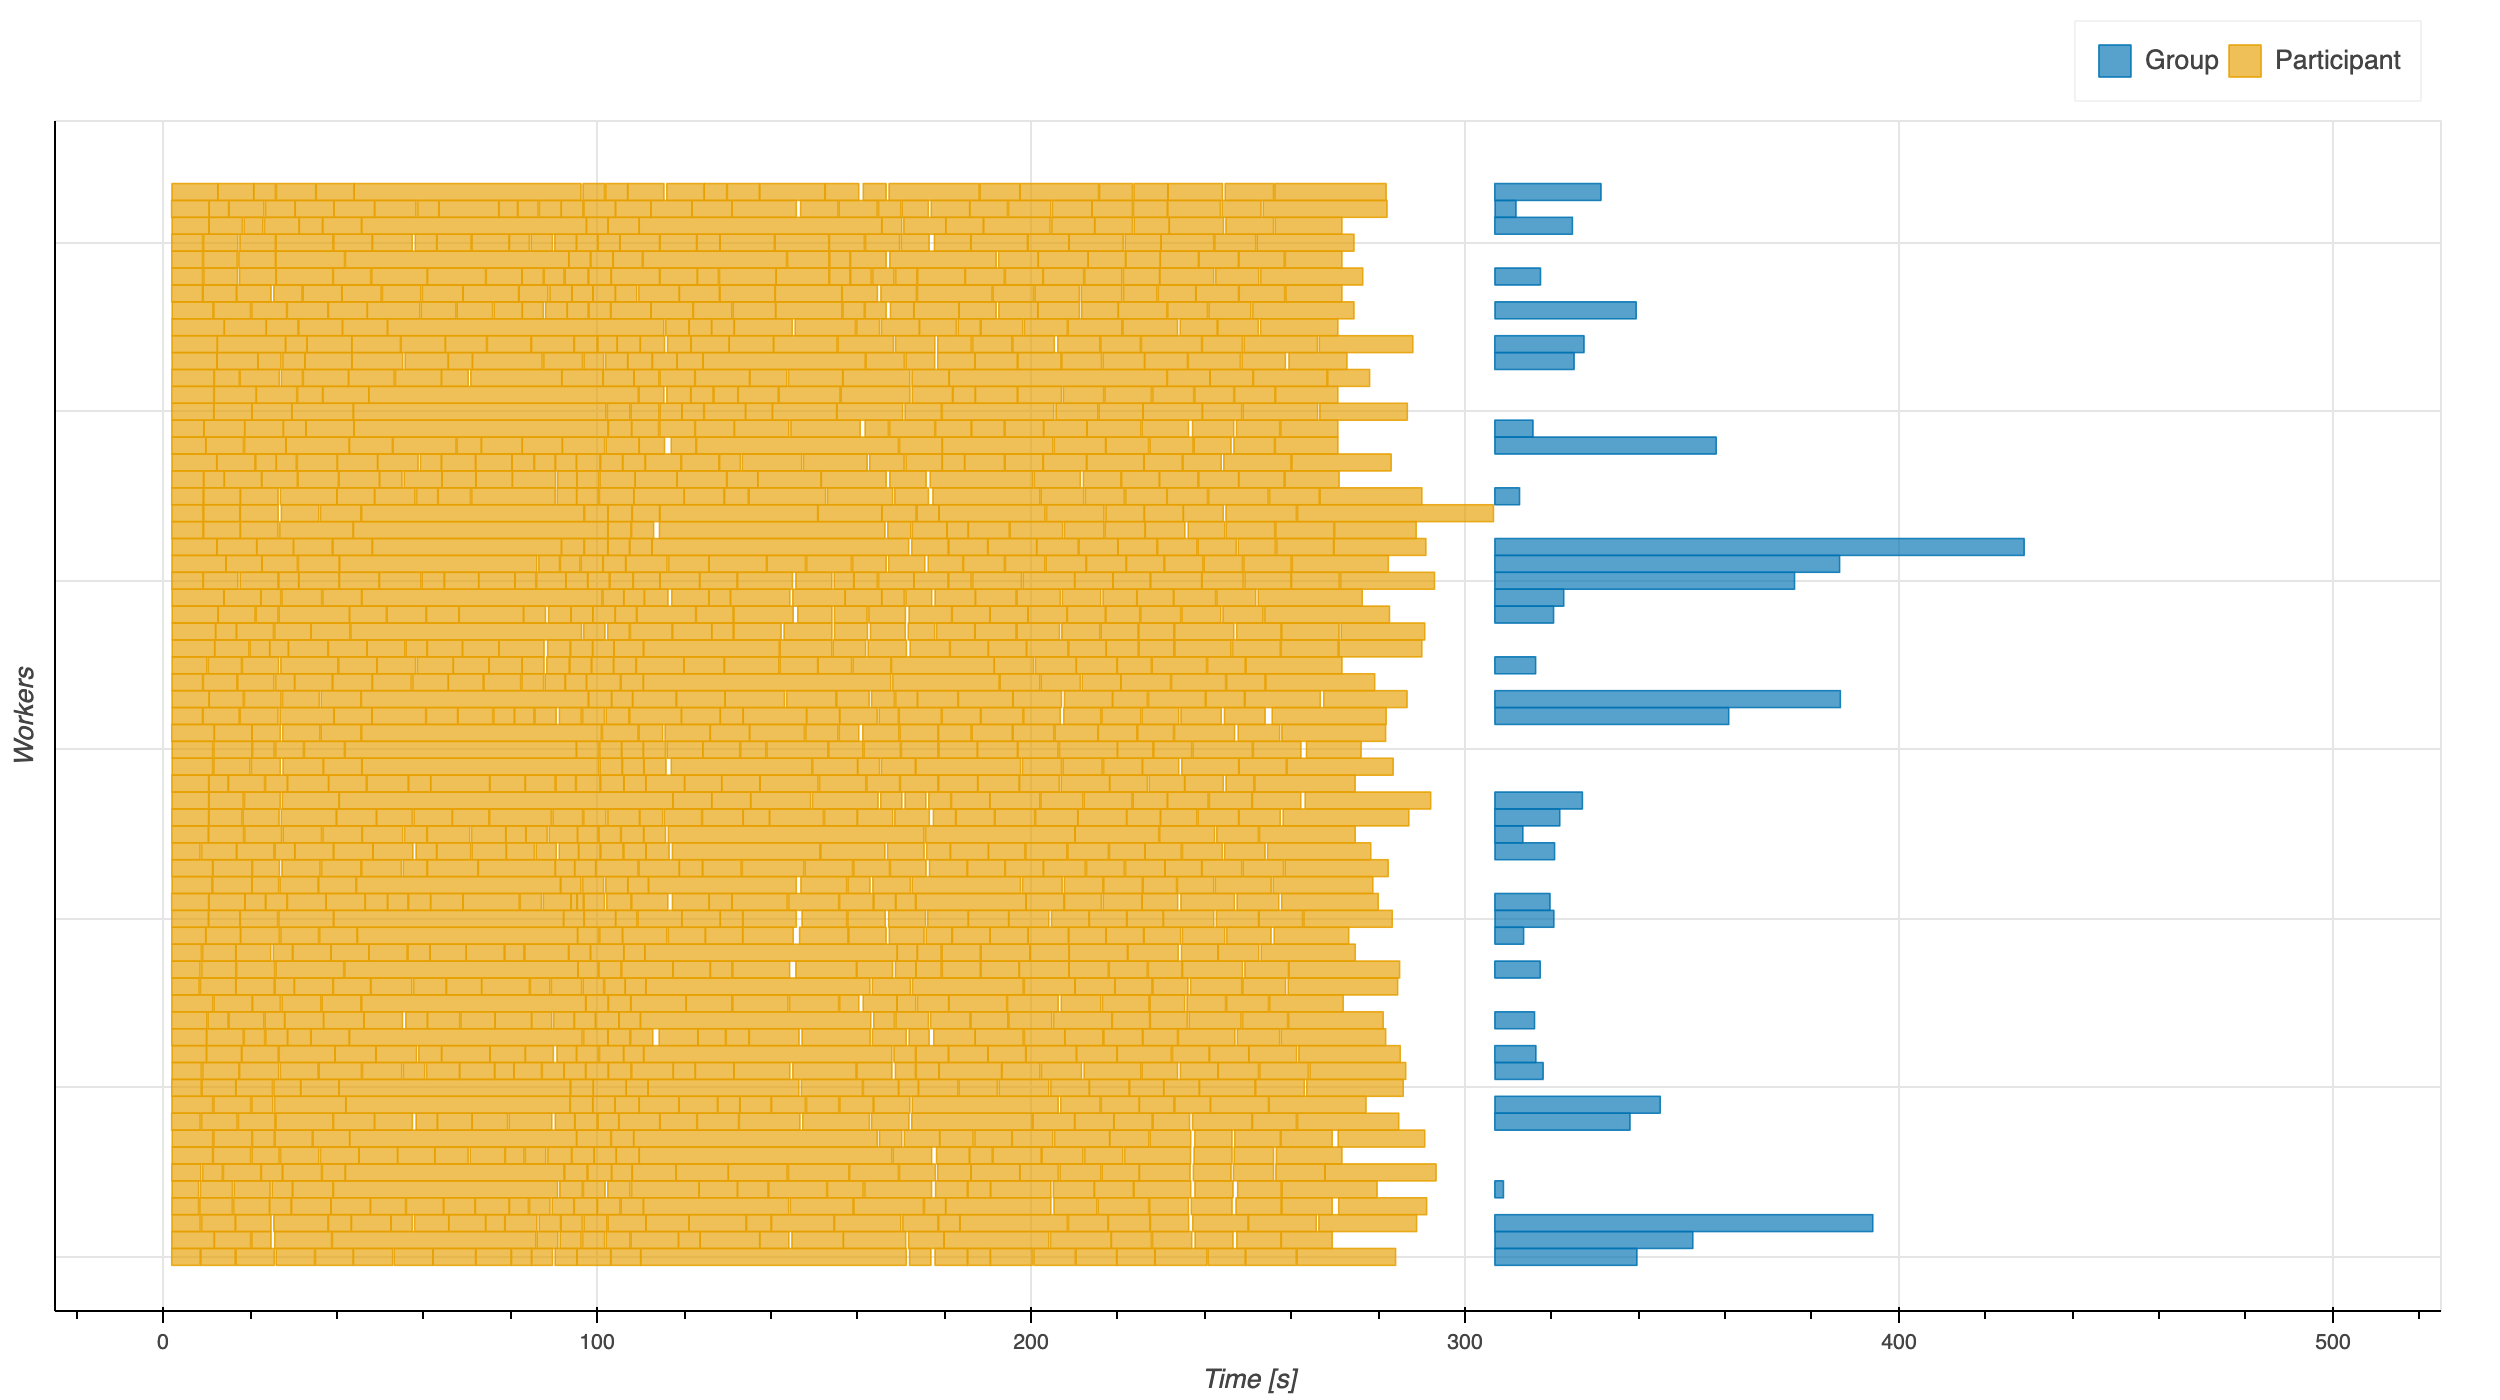
\includegraphics[clip,width=\columnwidth,
        height=0.15\textheight]{images/bag_bids_gantt.png}}
        \caption{Dask Bag}\label{fig:bids_dask_bag_gantt}
    \end{subfigure}
    \\
    \begin{subfigure}[b]{\columnwidth}
        \href{https://zenodo.org/record/3354434/files/dask-delayed-bids-baseline.html?download=1}{
        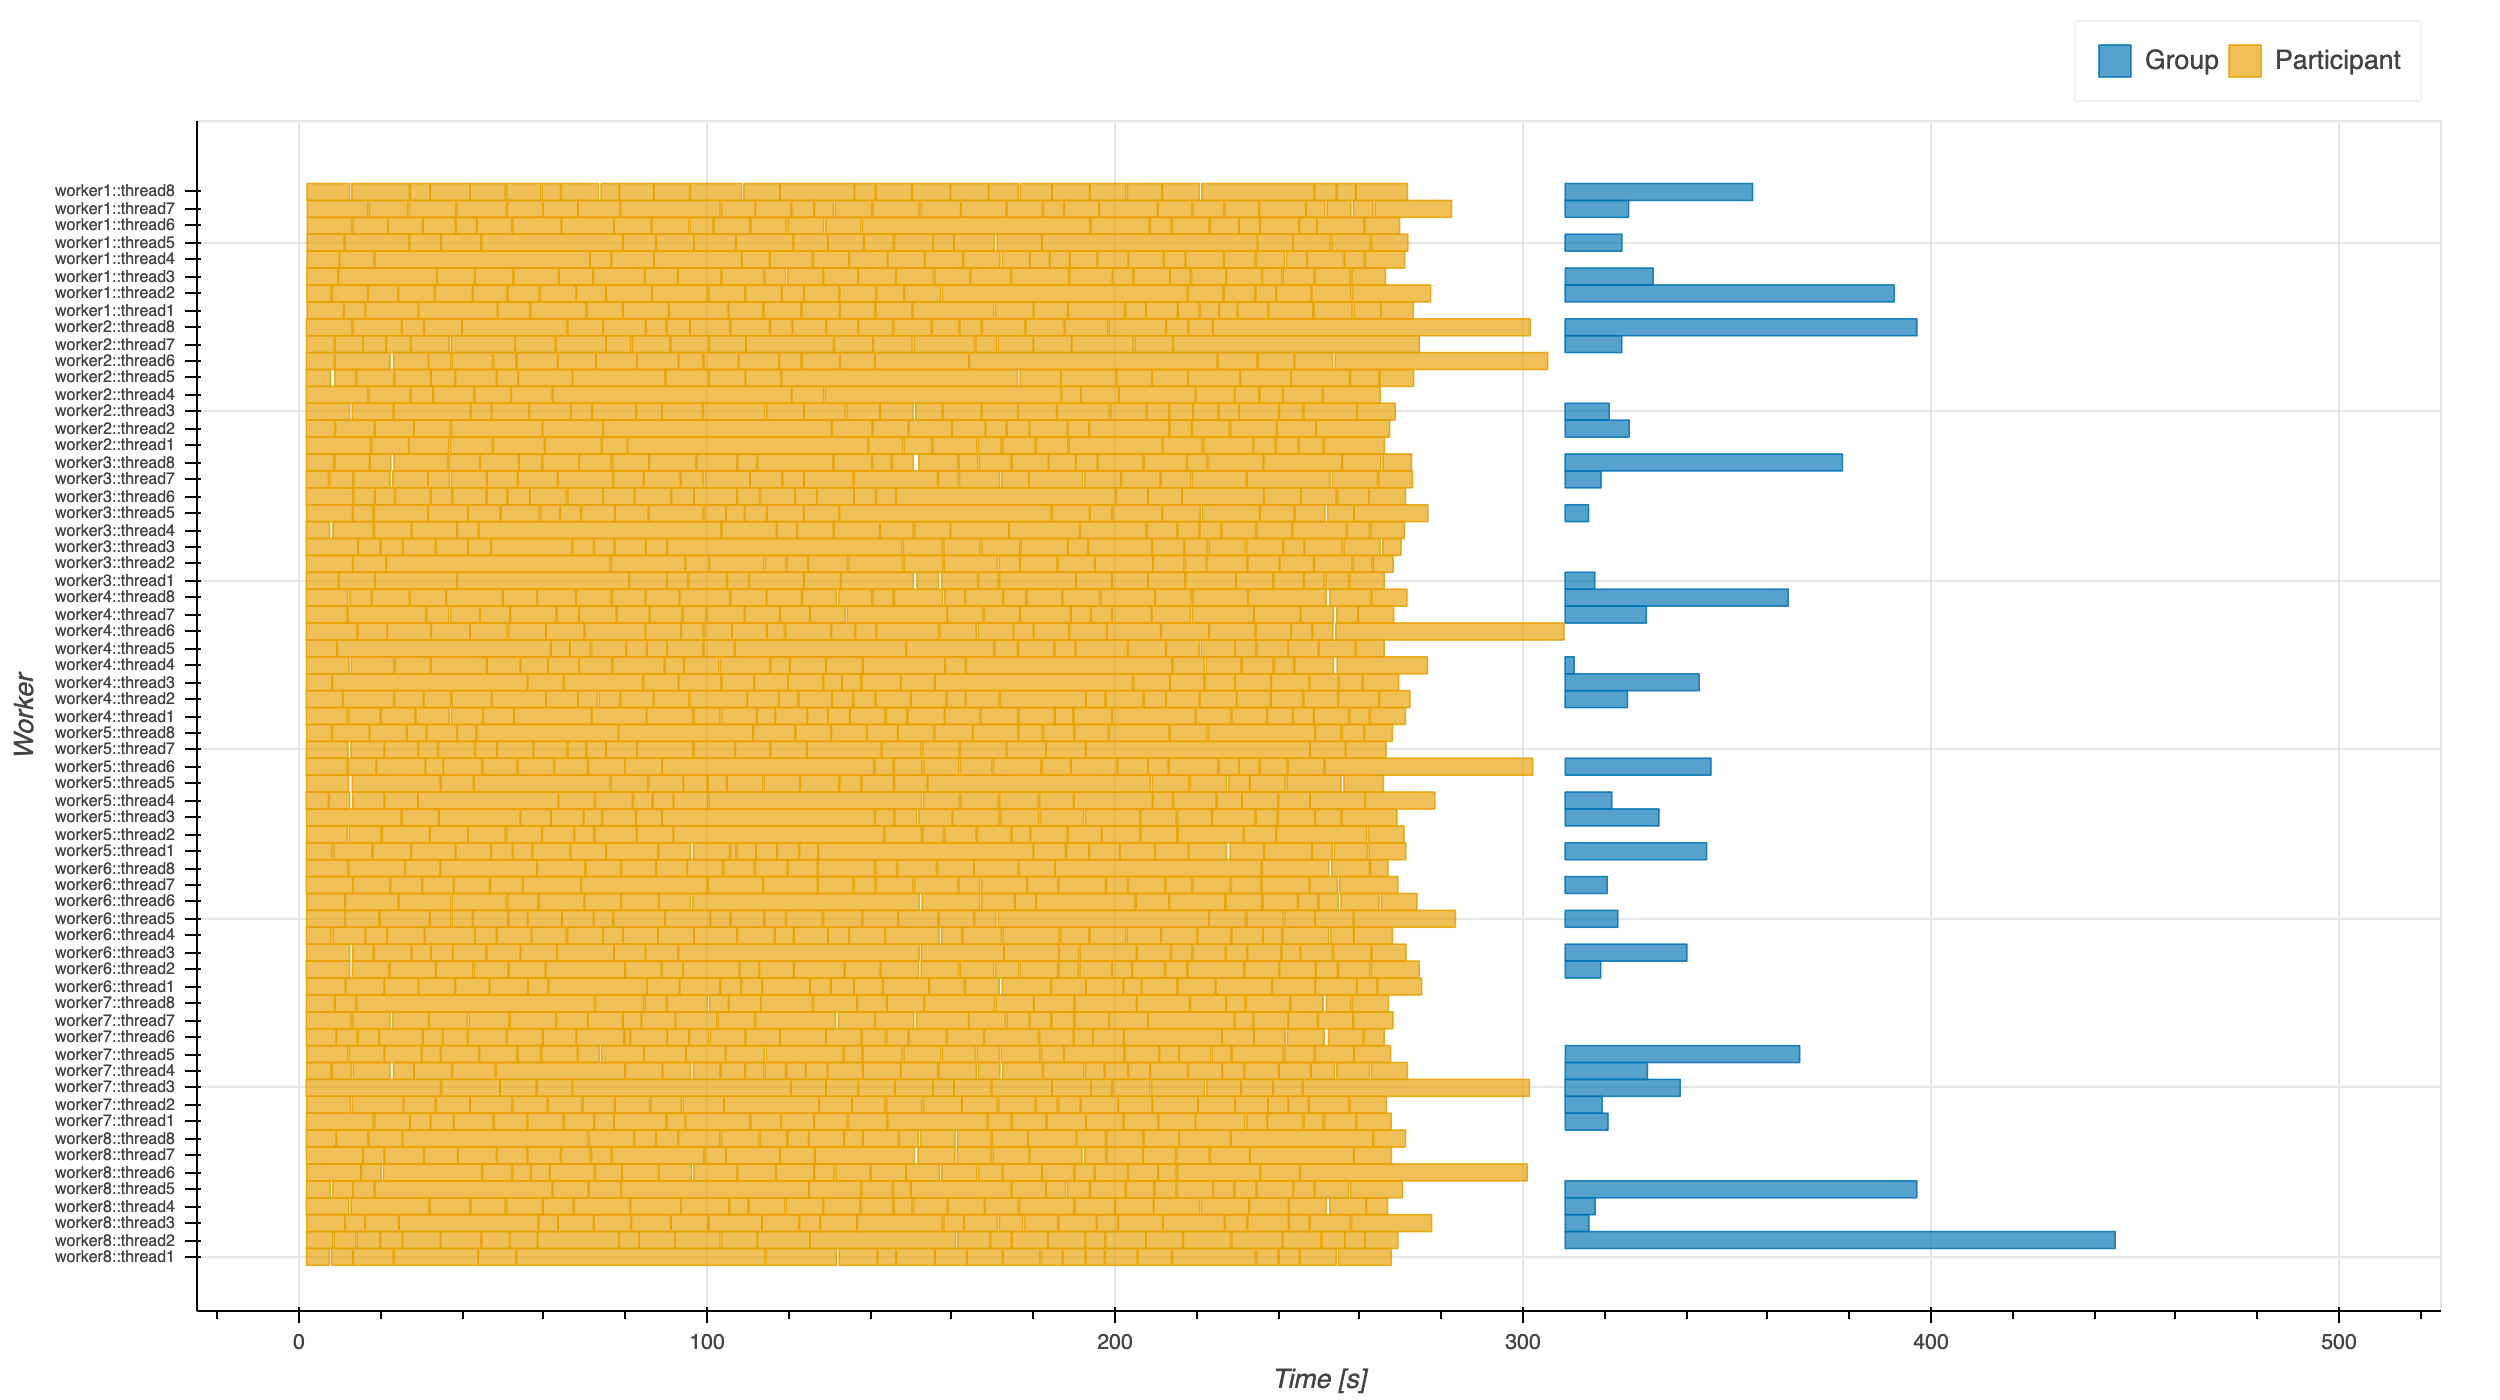
\includegraphics[clip,width=\columnwidth,
        height=0.15\textheight]{images/delayed_bids_gantt.png}}
        \caption{Dask Delayed}\label{fig:bids_dask_delayed_gantt}
    \end{subfigure}
    \\
    \begin{subfigure}[b]{\columnwidth}
        \href{https://zenodo.org/record/3354434/files/dask-futures-bids-baseline.html?download=1}{
        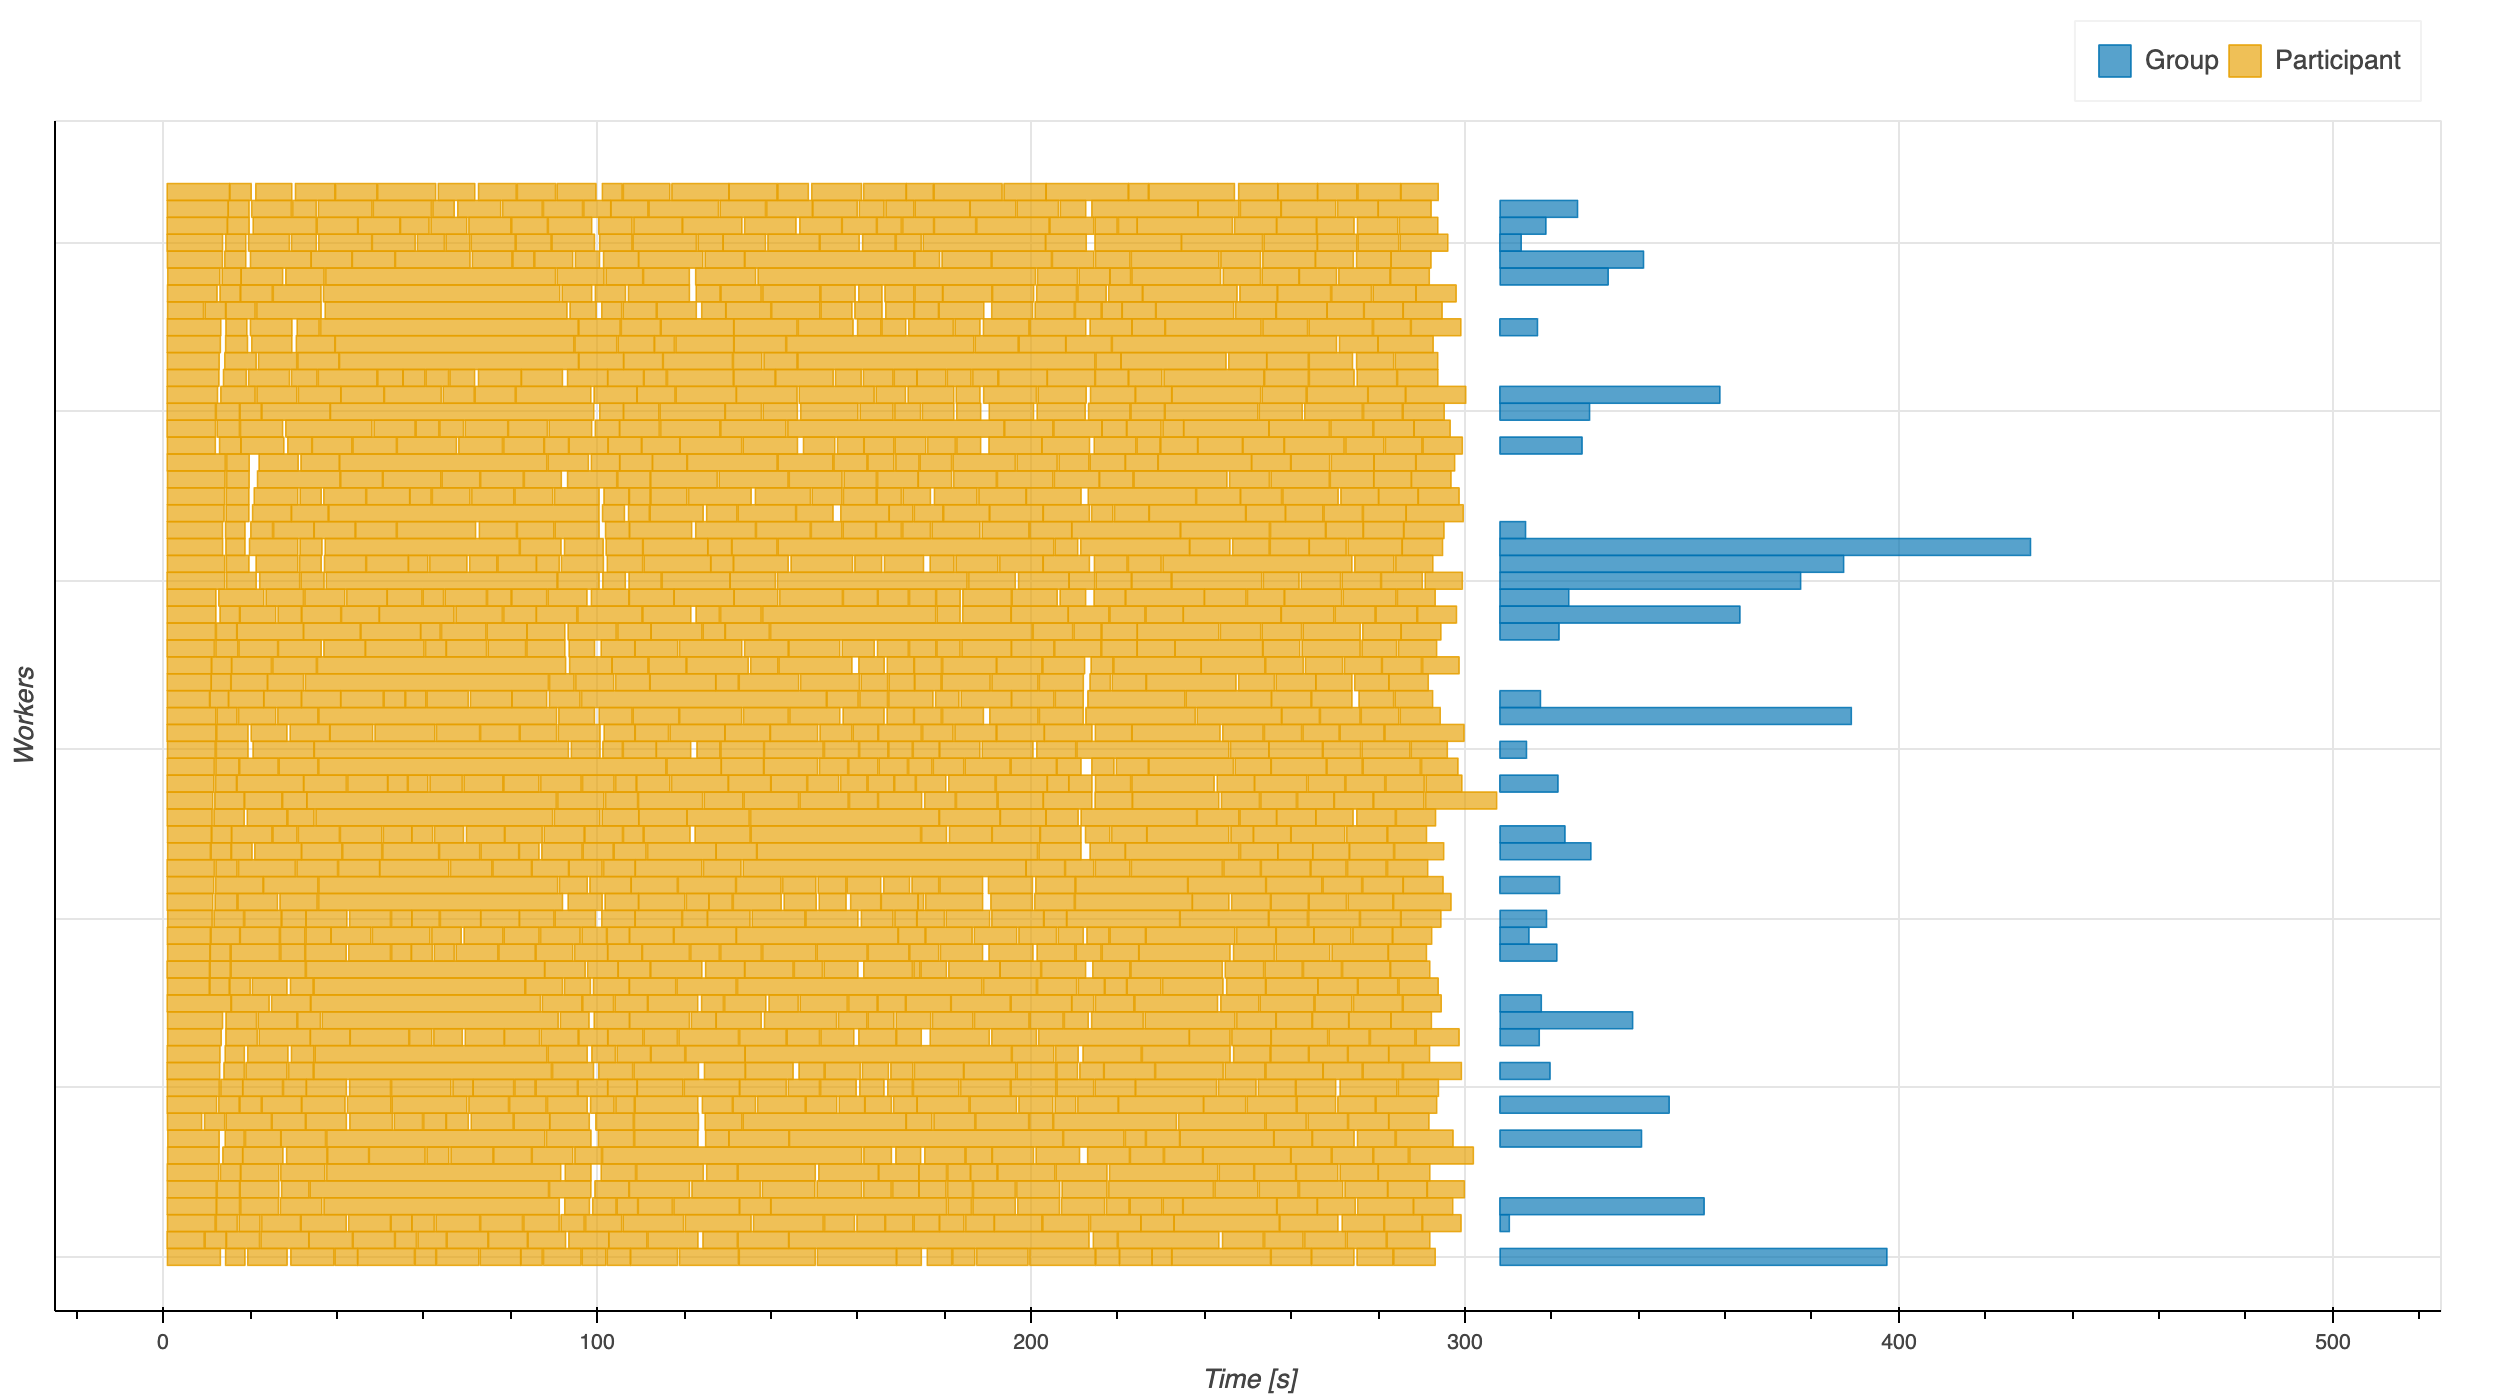
\includegraphics[clip,width=\columnwidth,
        height=0.15\textheight]{images/futures_bids_gantt.png}}
        \caption{Dask Futures}\label{fig:bids_dask_futures_gantt}
    \end{subfigure}
    \caption{BIDS App example: 8 workers}\label{fig:bids_gantt}
\end{figure}



%%%%% DISCUSSION %%%%%
\section{Discussion}

\subsection{Effect of Network File System}
We used an NFS as it is a common approach to store a large amount of data. However,
it limits the available bandwidth since all workers interact with one disk. This
causes data-intensive applications to take a significant amount of time for IO. As we
expect, this effect is amplified when too many tasks simultaneously try to operate
with the NFS at the same time as
Fig.~\ref{fig:inc_gantt},\ref{fig:histo_gantt},\ref{fig:histo_np_gantt},\ref{fig:bids_gantt}
shows. A parallel file system, such as Lustre~\cite{lustre}, would likely improve
IO times of parallel applications simultaneously writing to shared storage.

\subsection{Effect of data-intensive applications}
In our experiments, Incrementation, Histogram (NumPy) and Histogram for Spark have
low compute time while BIDS App example and Histogram for Dask have significantly
longer compute time. When adding additional workers, we observe that the highly
data-intensive applications scale poorly while compute-intensive applications scale
almost linearly This is due to the limitation from the NFS, as mentioned above.

Data transfer accounts for the majority of the execution time for data-intensive
applications (see
Fig.~\ref{fig:inc_gantt},\ref{fig:histo_spark_gantt},\ref{fig:histo_np_gantt}). We
see that when a low number of IO tasks are overlapping, this diminishes the bandwidth
limitation from the NFS. We want to explore solutions to desynchronize IO tasks in
the aim to reduce the makespan of data-intensive applications.

\subsection{Effect of the Global Interpreter Lock}
Python's GIL prevents multi-threading in Python. Dask tries to minimize the
consequences of the GIL by using external Python extensions. We found that Dask has
issues to parallelize Python functions while Spark did not (see
Fig.~\ref{fig:histo_tt_worker}). However, Dask was easily able to parallelize
application with functions in Numpy (see
Fig.~\ref{fig:inc_tt_worker},\ref{fig:histo_np_tt_worker}) and command-line
applications (see Fig.~\ref{fig:bids_tt_worker}). This is because, for Dask, the
instances are configured to have 1 worker process with 8 threads. Since the Histogram
implementation does not release the GIL it can only use one of the thread at a given
time thus it slows down the computation significantly.

One should be careful to configure the workers properly depending on the type
of functions executed in an application.

\subsection{Effect of tasks' size}
We measured the effect of various block sizes for constant BigBrain image for
Incrementation, Histogram, and Histogram (NumPy). We observe that larger block size
results in more IO compensated by lower overhead time. On the other hand, smaller
block size results in higher overhead time compensated by reduced IO time.

The number of partitions also has an impact on the size of the tasks. We set a
partition for each block or subject. There is a trade-off for the number of
partitions. On the one hand, a low amount of partition results in larger tasks thus
in lower scheduling overhead. On the other hand, a higher number of partition
results in smaller tasks hence more tasks fit in the workers' memory insuring that
they always have something to work on.

Varying the block size is equivalent to varying the size of the partitions. We
observed no difference when varying the task size while using an NFS. However, if
one uses a parallel shared file system, we suppose it would be preferable to use a
larger block size as the IO time should be reduced substantially. It is worth noting
that the Dask developers suggest, in
\href{https://docs.dask.org/en/latest/best-practices.html}{Dask's best practices}, to
use a partition size such that workers have 2-3 times as many chunks available to
work on. More experiments would have to be performed to gain insight on an optimal
number of partitions to use for a given set of data-intensive applications.

\subsection{Other comments}
Spark performance should be reduced by the serialization of Python functions to Java,
however, our results show no significant impact of it. 

Previous work showed that Dask has a the largest start-up overhead~\cite{Mehta:17}
when processing few subjects. Our Gantt charts show that Spark has a higher start-up
overhead. We think this is due to the larger amount of subjects we process.

The same study showed that Dask has a lower end-to-end runtime than Spark in a
neuroimaging analysis application. In our results, there is no significant difference
between the engines. We think this is because the applications we chose are highly
data-intensive while the one used in their study is compute intensive.

\section{Conclusion}
We presented a comparison of two Big Data engines, Apache Spark and Dask.
We studied the engines on three data-intensive neuroimaging applications
representative of common use cases. Our results show no substantial
performance difference between the engines, except for compute-intensive
Python applications where Dask is slower than Spark due to parallelism loss
coming from Python's Global Interpreter Lock. Interestingly, differences in
engine overheads do not impact performance due to their impact on data
transfer times: higher overheads are almost exactly compensated by a lower
transfer times when data transfers saturate the bandwidth. These results
suggest that future research should focus on strategies to reduce the
impact of data transfers on applications.

\section*{Acknowledgment}

Mathieu Dugr\'e was funded by an Undergraduate Student Research Assistant award from
the National Science and Engineering Research Council of Canada. We warmly thank
Compute Canada and its regional center Westgrid for providing the cloud infrastructure used in
these experiments, and the McGill Center for Integrative Neuroscience for giving us
access to their cloud allocation.

\bibliographystyle{IEEEtran}
\bibliography{IEEEabrv,reference}

\end{document}
